% Complementary Threat Knowledge in Federated Android Malware Detection
% LaTeX rendering of the chapter manuscript (APA 7 manuscript layout).
% NOTE: IGI Global accepts Microsoft Word (.docx) submissions only; this source is for editing/preview.
\documentclass[12pt,letterpaper]{article}
\usepackage[T1]{fontenc}
\usepackage[utf8]{inputenc}
\usepackage{newtxtext,newtxmath}
\usepackage[margin=1in,headheight=15pt]{geometry}
\usepackage{setspace}
\usepackage{microtype}
\usepackage{graphicx}
\usepackage{booktabs,tabularx,array,makecell}
\usepackage[font=normalsize,labelfont=bf,textfont=it,labelsep=newline,justification=raggedright,singlelinecheck=false,skip=6pt]{caption}
\captionsetup[table]{position=top}
\captionsetup[figure]{position=top}
\usepackage{titlesec}
\usepackage{fancyhdr}
\usepackage{newunicodechar}
\usepackage{xurl}
\usepackage{indentfirst}
\usepackage[hidelinks]{hyperref}

\newunicodechar{−}{\ensuremath{-}}
\newunicodechar{±}{\ensuremath{\pm}}
\newunicodechar{×}{\ensuremath{\times}}
\newunicodechar{≥}{\ensuremath{\geq}}
\newunicodechar{μ}{\ensuremath{\mu}}

% APA 7 manuscript: double spacing, 0.5in paragraph indent, no extra paragraph space
\doublespacing
\setlength{\parindent}{0.5in}
\setlength{\parskip}{0pt}
\frenchspacing
\raggedbottom
\widowpenalty=10000
\clubpenalty=10000

% APA headings: level 1 centered bold; level 2 flush-left bold
\titleformat{\section}{\normalfont\bfseries\centering}{}{0pt}{}
\titleformat{\subsection}{\normalfont\bfseries}{}{0pt}{}
\titlespacing*{\section}{0pt}{\baselineskip}{0pt}
\titlespacing*{\subsection}{0pt}{0pt}{0pt}

% page number top right
\pagestyle{fancy}
\fancyhf{}
\fancyhead[R]{\thepage}
\renewcommand{\headrulewidth}{0pt}

% floats: single-spaced content, table/figure notes below
\makeatletter
\g@addto@macro\@floatboxreset{\singlespacing}
\makeatother
\setlength{\textfloatsep}{12pt plus 4pt minus 2pt}
\setlength{\intextsep}{12pt plus 4pt minus 2pt}
\renewcommand{\topfraction}{0.9}
\renewcommand{\bottomfraction}{0.8}
\renewcommand{\textfraction}{0.07}
\renewcommand{\floatpagefraction}{0.75}
\newcommand{\notes}[1]{\par\vspace{4pt}{\footnotesize\raggedright\textit{Note.} #1\par}}

% references: hanging indent 0.5in
\newenvironment{references}{\begin{list}{}{\setlength{\leftmargin}{0.5in}\setlength{\itemindent}{-0.5in}\setlength{\itemsep}{0pt}\setlength{\parsep}{0pt}\setlength{\topsep}{0pt}}\raggedright}{\end{list}}

\urlstyle{same}
\renewcommand{\arraystretch}{1.15}
\hypersetup{pdftitle={Complementary Threat Knowledge in Federated Android Malware Detection},pdfauthor={Salaheddine Naslouby, Mohamed Lachgar, Hamid Hrimech}}

\begin{document}
\thispagestyle{fancy}
\begin{center}
\vspace*{1.5in}
{\bfseries Complementary Threat Knowledge in Federated Android Malware Detection}\\[0.5\baselineskip]
{\itshape A Controlled-Exposure Study}\par\vspace{\baselineskip}
\begin{singlespace}
\textbf{Salaheddine Naslouby}\textsuperscript{1,*}\textbf{, Mohamed Lachgar}\textsuperscript{2}\textbf{, Hamid Hrimech}\textsuperscript{1}

\vspace{0.6\baselineskip}
\textsuperscript{1} Hassan First University\\
National School of Applied Sciences (ENSA), LAMSAD Laboratory\\
Berrechid, Morocco

\vspace{0.6\baselineskip}
\textsuperscript{2} Cadi Ayyad University\\
Higher Normal School (ENS), L2IS Laboratory\\
Marrakech, Morocco

\vspace{0.6\baselineskip}
* Corresponding author: Salaheddine Naslouby\\
Email: \href{mailto:naslouby.salahe@gmail.com}{naslouby.salahe@gmail.com}; ORCID: \href{https://orcid.org/0009-0002-7295-7816}{0009-0002-7295-7816}

\vspace{0.6\baselineskip}
Mohamed Lachgar: \href{mailto:m.lachgar@uca.ac.ma}{m.lachgar@uca.ac.ma}\\
Hamid Hrimech: \href{mailto:hamid.hrimech@uhp.ac.ma}{hamid.hrimech@uhp.ac.ma}
\end{singlespace}
\end{center}
\clearpage

\section*{Abstract}

\noindent We can learn from more data or even learn from families we do not have access to locally when using collaborative malware detection methods. This chapter breaks down what each can contribute by exposing our clients to different families. We did this with four custom built Android app domains. Using partitions that are aware of the groups used in our experiments we train on the same amount of samples for every exposure setting and use per client thresholds and 10 seed confirmations. When our FPR was 5\% Federated Average training where our clients have other families present learns 11.96 percent more unseen families (95\% CI [9.15, 15.21]) than no families being present everywhere. We estimate a collaboration effect of 1.51 points which has an uncertainty that includes 0. Our clients will learn 3.26 percent more unseen families on their own domain malware when other families are present than learning locally. However they will detect 3.61 less nonhidden-malware. When extending to new seeds we find that our wrong family placebo will barely recover any gains and that complementary gain grows with the number of families your peers know. Comparing local vs federated learning is not enough to see how many families our peers must know to get these gains.

\clearpage

\section*{Introduction}

It is possible for an Android malware detector to have many training samples but be missing from a family of concern. It simply may not have any examples for a particular family. Applications are collected from many sources and have different families, benign apps and classifications. There will come a time that the detector will have to detect a family that was never shown to it during training. Other clients may have those examples but how do we know if working with others will help you detect that family better than working with other information you have access to.

Federated Learning allows models to be trained on multiple datasets by combining parameters that are learned from each local client. By averaging the local clients weights we can create one average model (McMahan et al., 2017). If you were to compare a federated model to a local model there are many factors that could affect your outcome. From number of clients you train with to different families you are exposed to. It becomes difficult to attribute federated models success to your peer clients. What if your overall performance drops but you gain the ability to detect more families that were not represented on your client.

We define Complementary Threat Knowledge (CTK) with the following variables. There is a family chosen that is not shown to our client of interest. Our baseline for this would be the local client. When collaborating with peers we cannot show those hidden families or we can have those families on our peer clients. We measure CTK by finding the difference between our recall score with families on peers and without any of the families hidden on all clients. We call the difference between no family hidden and the local detector pooling. These two values will break down the recall difference we find between having the hidden families on peers vs the local detector. CTK represents the recall gain from having these families on your peers.

We want to measure if your model can learn more families than it has been exposed to by using collaboration. We can use collaboration to pool these extra families and see if that increases your recall scores. It is also possible that by pooling other malware families your recall scores go down. And the complementary exposure can make up for that allowing your model to perform similarly to your local model. By reporting these three numbers we can see what families you gained from having others collaborate with you and if it has an impact.

We use the LAMDA features along with metadata from AndroZoo to create four different markets/time periods to be our clients. We can then measure binary classification against families that were removed from our clients of interest. Using the benign apps from each client we can threshold our detectors. Packages will not cross the fit/cal/test lines and we won't have identical first level features appear across the lines. We believe our methods allow us to evaluate if your model can learn families it was never trained on by collaborating with others.

By looking at our 10 seeds of confirmation we show an increase of 11.96 (95\% BCa CI 9.15–15.21) percentage points in recall for families we did not show to the model across all clients of a federated setup. We are able to break this down from increasing recall on families within our domain and look at decreases in recall for nonhidden malware families. We also look at our clients individually and families to see where we may have lost.

Our contribution is to show a framework for finding increased detections when working with peers on detecting Android Malware. By creating clients that have similar budgets and manipulating the families your models see. You can see if by working with peers you increase your detection rates above your local model. We then go further to look at families and clients we may have failed on and show why collaboration works in our case. Using current state of the art learning algorithms we can test if having your peers collaborate will allow you to detect new families or just recover from collaboration.

All differences in recall are in percentage points. Recall and false positive rates are shown as a percentage. We will refer to nominal FPR as the FPR we tried to achieve on calibration and the actual FPR on our test set of benign applications. Intervals will be 95\% BCa for our means unless stated otherwise.

\section*{Background and Related Work}

\subsection*{Android Malware Detection and Family Generalization}

Applications have been represented and classified to discover malware on Android for some time. By representing applications with manifest and code static features such as permissions and APIs. As well as having an explanation of which features identify them as malicious (Arp et al., 2014). Allowing fast comparisons over sets of applications. And demonstrates how families can be learned from each other when the problem being classified is malware or not. Families are held out from training in the CTK-Android setting and decide what we would like to test. Learning to classify if an app is malware can generalize to a family that is locally unseen. Before collaboration occurs.

How you represent your problem will allow for more or less commonality to be discovered. MaMaDroid takes APIs and builds Markov chain representations to classify them (Mariconti et al., 2017). API package's or families are generalized in a similar fashion to what malware families could be held out. But does not mean they are held out for learning. There may be a common pattern that malware family shares that can be discovered with another type of representation. Not showing improvement with your chosen representation of the problem does not imply that it can't be learned. When comparing CTK with other methods you need to take into account how the representation was extended. Not just how many additional features were added.

Using family annotations can lead to ambiguity when trying to learn what has been exposed. Many methods have taken steps to better extract what malware families an application is. AVClass2 uses a predefined set of tags and rules to decipher anti-virus families (Sebastián \& Caballero, 2020). Some datasets have used automated family detection to create their dataset. While this is helpful when deciding what to expose during a learning environment. We can't assume they are all correctly labeled as they are malware families. They may all use an ad service or be related to each other in some form. When learning with CTK-Android we learn with what family annotations are given.

\subsection*{Federated Learning and Complementary Exposure}

FedAvg aggregates the models locally learned each round. FedProx limits how much each client deviates from the aggregated model using a proximity term (Li et al., 2020). We use these approaches as our comparison points. As their aggregate functions may have client compromises when dealing with missing Android families we test how these improve upon it.

There has been some research into this. Ciaramella et al. (2026) looks at comparing federated malware detection to centralized approaches. Using app code images with Convolutional Networks they can compare various factors such as how data is distributed across clients. How the data is aggregated among others. Gálvez et al. (2021) explores privacy with classification in a FL system and Patel et al. (2026) tackles changing concepts on the client level. M2FD uses Federated learning for mobile malware detection and monitors for drift to retrain certain models with KronoDroid (Augello et al., 2025). Droidware focuses on more static features and builds off FL by adding authenticated models as well as outlier checks (Prasad \& Kumar, 2026). This gives us more insight on these types of systems that may face these problems in the real world. Our experiment aims to compare differences between the client exposure.

There are similar challenges found in other cybersecurity domains. Ongun et al. (2025) created a Federated learning method called CELEST to detect HTTP based cyber threats across multiple networks. They can measure how well a federated detector performs if there are threat families on the network but not on the client level. CELEST creates controlled testing situations to also include an active learning algorithm and protection against malicious nodes. Our approach adds on to this with matching number of missing samples on every client. And measures recall with many classes of interest. With a seed randomization to measure error bars. Although CELEST looks at many facets that could be applied to our system we do not go into those topics here.

A similar concept is used in CyberForce. Which varies how many clients do not have a specific malware type present (Feng et al., 2025). Testing this through Federated Reinforcement learning to detect malware on IoT devices. It shows similar results by having an instance where all clients are missing the target class. Comparing to a reference at the client level. With varying aggregation algorithms as well. While this problem may differ from Cyberforces approach by looking at Moving target defense. By varying how many clients are missing a specific malware. We take inspiration from them and add onto their work by implementing the same methods as CyberForce with Android Devices. Ensuring that each client has the same amount of the target class present. As well as implementing a wrong class dose to our clients.

By implementing missing class problems in machine learning can show us how our model performs without the ability to detect that class. There are works that explore missing classes as well (Shen et al., 2024). Showcasing their model on intrusion detection. By lacking one class per client they see if they can learn from their neighbors. Popoola et al. (2022) explore a similar problem of missing unseen bots. We take inspiration from their idea that missing a class can impact your model and test how far away you can get from detecting the class. Just like Shao et al. (2026) showed that your model can converge and still have bias due to lack of positives.

\subsection*{Dataset Quality and Evaluation Validity}

AndroZoo offers many apps with metadata that allows researchers to look deeper into datasets outside of the typical small sets of malware (Allix et al., 2016). With metadata we are able to construct good domains however we only use this as an observed value. By using only one market field we will be limiting our set of apps but know for sure what market field they belong to. If we take those domains that were kept and create a federation out of them we are only creating a benchmark. Not knowing if those market fields would behave like actual defenders when working together.

There have been recent efforts to collect data on Android benchmarks that span across more time. Allowing for drift analysis (Haque et al., 2026). Also work was done to align data across multiple forms of collection on the same apps over time (Kamol et al., 2026). While these works help decide on our choice for a dataset and how to represent the apps. They don't focus on the problem we are trying to solve in CTK-Android. When working with LAMDA we used the version of the dataset with 925 features. We do not assume all versions of LAMDA have 925 features. We can also compare how we represented the apps with McNdroid since there is overlap.

Research has shown that we can get skewed results when looking at time and space with classifying malware (Pendlebury et al., 2019). There are many issues to keep in mind when working with malicious app data. Some include how you collect your data, leaking information from training to test data and more (Arp et al., 2022). Our goal with CTK-Android is to address data leak due to identical apps. And address the problem of not knowing if data comes from collaborating parties. We don't enforce any ordering of time when we split up our clients by date. Research has also looked into chronological order when working with Android data and FL (Patel et al., 2026). We can address this by having groups and exposing each to a threat.

We address the problem of matching budgets when detecting threats in Android federated learning. By having a local arm we can see how much our peers are helping us detect a threat. Then comparing our local arm to a group with the threat present and no threat. We can further see how our clients react to each other when working together on missing threats.

\section*{Research Problem and Questions}

A seed specifies a group-aware partition and selected families' target assignments. For learner $m$, $R(m,P)$ is a specified recall metric when targets lack their assigned families and peers retain them; $R(m,A)$ is the same metric when all selected hidden families are absent from every client's fit data. $R(L,P)$ is the recall of the local learner on the same target-family task, although peer data do not enter its training. All quantities share the seed, nominal operating point, and evaluation population:
\begin{gather*}
\mathrm{CTK}(m) = R(m,P) - R(m,A) \\
\mathrm{Pooling}(m) = R(m,A) - R(L,P) \\
\mathrm{Total}(m) = R(m,P) - R(L,P) = \mathrm{CTK}(m) + \mathrm{Pooling}(m)
\end{gather*}

They will exist in each paired set of seeds prior to averaging across effects. It is possible for both CTK and pooling to be less than 0. Both forms of exposure involve using the same learner, number of training epochs and amount of clients for each family. By withholding families we change the replacement examples. So CTK is our measure of how well our model was able to learn from this effect. Since we withhold multiple families in one run a family will be affected based on what other exposures occurred. Similar to CTK pooling will have differing training methods. With FedAvg we train for 20 rounds with 2 local epochs. Our local baseline will train for 10 epochs. We will see some gain from this as well and should not all be attributed to more data.

Does our exposure to other families help our model recognize unseen families once pooling is taken out? This is our first question. Our main interest is in unseen family recall using FedAvg across all families at nominal FPR of 5\%. Second is how much will our model benefit from being exposed to other families. We can see how this varies between families and target clients. Maybe the model learns from another family that allows it to overcome its poor performance from pooling. Our third question involves learning strategies and cutoff values. Recall for unseen families should be viewed with recall on nonhidden malware, actual FPR and lowest client. Fourth will our results stand if we vary the way we split our families, number of supporting clients, number of families, model architecture and features. All these questions are important but can provide different types of evidence. We may find that there is a wide range of gains and not all of that will be our next confirmatory question.

Using all families will improve our withheld clients given the same constraints on budget and learner. This is only our lower bound because a model could surpass this if sampled properly and given enough optimization time. The ratio we will see later of additional headroom recovered by our exposure will use the full exposure centralized recall. The family level tables may have the same learners full exposure recall. Keep in mind these values are not the same.

As stated before CTK and Pooling will be divided by their respective means over the mean gain. Both shares are greater than 1 when their opposing counterpart is less than 0. Shares can have extreme variance when total gain approaches 0. Our testing scenario will need enough gain to create an interval around our share. Again recall differences will be the best descriptors when there is offsetting gain and loss.

\section*{Controlled-Exposure Study Design}

\subsection*{Data Sources and Constructed Clients}

There are 1,008,381 rows of applications in our chosen source with 925 columns of static features. This source comes from the LAMDA var\_thresh\_0.01 release. We will be taking the feature columns provided and have any that have a positive value will be turned into a column to check if the app has that feature or not. There will be no extra feature finding or vocabulary built in this chapter. Our source states that if an application is detected by 4 or more viruses it is considered malware and if 0 detections it is considered not malware. We will not use apps that fall in between our stated labeling. LAMDA provides us with data from 2013–2025 with no apps from 2015 (Haque et al., 2026). This allows for our study to use different time frames but we will be creating our own train/test sets.

We match the applications to their respective SHA-256 on AndroZoo. Making sure there is only one link to metadata and matching virus total count. As stated in our link checking the 1,008,381 rows of applications were able to be linked to AndroZoo with no unmatched rows. Using the package name and markets will allow us to find matching ids and build our clients. We only want applications that are linked to one market so they can be assigned to our chosen markets. We will have Anzhi and AppChina as one client each. Apps that are found on Google Play will be split into two groups one being play-early (before 6/2019) and play-late (after 6/2019). All other applications will not be used in our four clients. Table~\ref{tab:1} shows the amount of applications we have in our data. There are 832,165 total applications with 257,564 being malware and 574,601 being not malware.

\begin{table}[!htbp]
\caption{Retained Applications in the Four Constructed Clients}\label{tab:1}
\small
\begin{tabular*}{\linewidth}{@{\extracolsep{\fill}}lcccc@{}}
\toprule
\textbf{Client} & \textbf{Applications} & \textbf{Malware} & \textbf{Benign} & \textbf{Malware (\%)} \\
\midrule
anzhi & 104,287 & 90,801 & 13,486 & 87.07 \\
appchina & 88,282 & 73,578 & 14,704 & 83.34 \\
play-early & 319,122 & 75,985 & 243,137 & 23.81 \\
play-late & 320,474 & 17,200 & 303,274 & 5.37 \\
\bottomrule
\end{tabular*}
\notes{Corpus counts before grouped splitting and fit-budget selection. Client labels denote constructed market/era domains; percentages describe this selected corpus.}
\end{table}

As displayed in Table~\ref{tab:1} each corpus has varying amounts of classes within it. There are more malicious apps on Anzhi and AppChina than there are benign. While there are less malicious apps than benign on both Google Play data sets. By allowing each dataset to have these proportions we are not forcing the same class amount to each client and allowing our global model to learn from various clients decisions. Which means if we increase our recall by an equal amount on each data set it may affect us differently. The percentages above are not what we believe to be the amount of malware currently circulating on these applications markets.

Each corpus is larger than what we used for fitting. For our main setting each client will fit 6,000 data points max for each arm and 1,500 for the lower support amount. Calibration and test data still have their partition groups left. Allowing us to have the same amount of data that was trained on during each collaboration but allow different proportions to be fit. So our peer support could be greater than what we use to fit.

\subsection*{Identity Grouping and Partition Construction}

There are two ways an app can be linked to another under our primary definition. They can have the same package name or the same feature vector (binary). We take connected components to be atomic. That means two apps could share a component via transitive closure of package names and features. Even if they don't share both package name and feature vector. These components will span our kept population meaning one identity could link apps with different clients. Components will have one assigned role for our whole study. We avoid matching primary feature vectors and packages between our fit, calibration and test data sets. While maintaining varied clients within each.

The expected percentage of apps in each role is 60\%/20\%/20\%. Given our seed we generate the order of the components along with a partition salt and attempt number. As we cumulatively add the length of each component we divide them into roles at their respective thresholds. Due to component being atomic our row percentages may not equal out to our expected percentage. For each seed and salt our code checks 16 attempts and keeps the largest number of fit client families and natural scarcity client families. If there is a tie we keep the first attempt. This is not based on how well they perform when trained it just finds the partition with the most support. Over our confirmatory seeds we get a range of 57–60 amount of eligible fit/natural scarcity client families. Which is larger than the median of 52.5–56 across all candidates. So our partition selection method helps us find partitions with about 9\% more support on average. Than our candidates it still conditions on this though which is a caveat to consider. When thinking about generality.

This leaves our initial partition method not time based. We define clients as early Google Play or late Google Play but both will have fit/cal/test sets. We are not able to claim that our app's date tells us if it was fit before it's tested. Our partition method is what will allow for this. As such we are measuring how well our model can generalize to new identities in the early/late Google Play sets. The only difference with our package only definition is that it has no identical feature linkage. This can help determine how dependent our method is on our chosen partitioning. But being consistent with our package only does not guarantee no forms of leakage.

\subsection*{Family Selection and Target Assignment}

When filtering families we do not include any of the empty/unknown/benign/singleton prefixed family names as possible targets. These filters apply only to our task of exposing families and do not mean all of these families were removed from binary learning. Any family that has at least 600 apps within our retained corpus and exist in at least 2 clients are allowed to become candidates. We then sort by support and use a deterministic ordering to select the top 8 alternating ranks between the primary and replication targets. This will yield families with reasonable support instead of picking a random group of families. Our primary set contains 8 names including frmy. The primary set for our controlled analysis will have 7 hidden families that meet our requirements. The replication will contain 8.

We require the following for a target family to be considered in our controlled target/family pair. There must be a minimum of 20 examples fitting the target that are held out. At least 150 fitting its peers. A total of 50 examples fitting the target in the entire fed and at least 500 examples left to fit the target. Once more families are added to a target this last value also holds for the sum of all previous targets. Clients are ordered randomly based on a seed and the first client that meets this condition becomes the target. Due to this each family may target different clients with different seeds. Support values used to determine candidate targets are measured before final amount removed. Target exposures must also meet these conditions where there is data left to train on peers.

Clients reporting own domain have a requirement of at least 15 hidden family test examples. This does not mean all hidden family/target pairs will meet this requirement in our controlled scenario. So while family selection is based on these conditions it should not be expected to return enough data in the own domain section. You will also notice the number of clients/seeds used in these reports differs. A family that is targeted could have low support in its own domain and still be included in federation wide results if it has high numbers of apps testing on other domains. Both of these scenarios are similar but different questions.

\subsection*{Exposure Conditions and Comparison Designs}

As shown in Figure~\ref{fig:1} we have our conditions for peer-present, absence-everywhere and full-exposure. Once excluded the order of our seeded clients determine what rows are chosen for training and whatever is available fills our budgets. This will give us the same amount of samples but may vary what data they consist of. Full exposure simply removes exclusion with the same budgets and timeframe.

\begin{figure}[!htbp]
\caption{Controlled Family Exposure Across Target and Peer Clients}\label{fig:1}
\centering
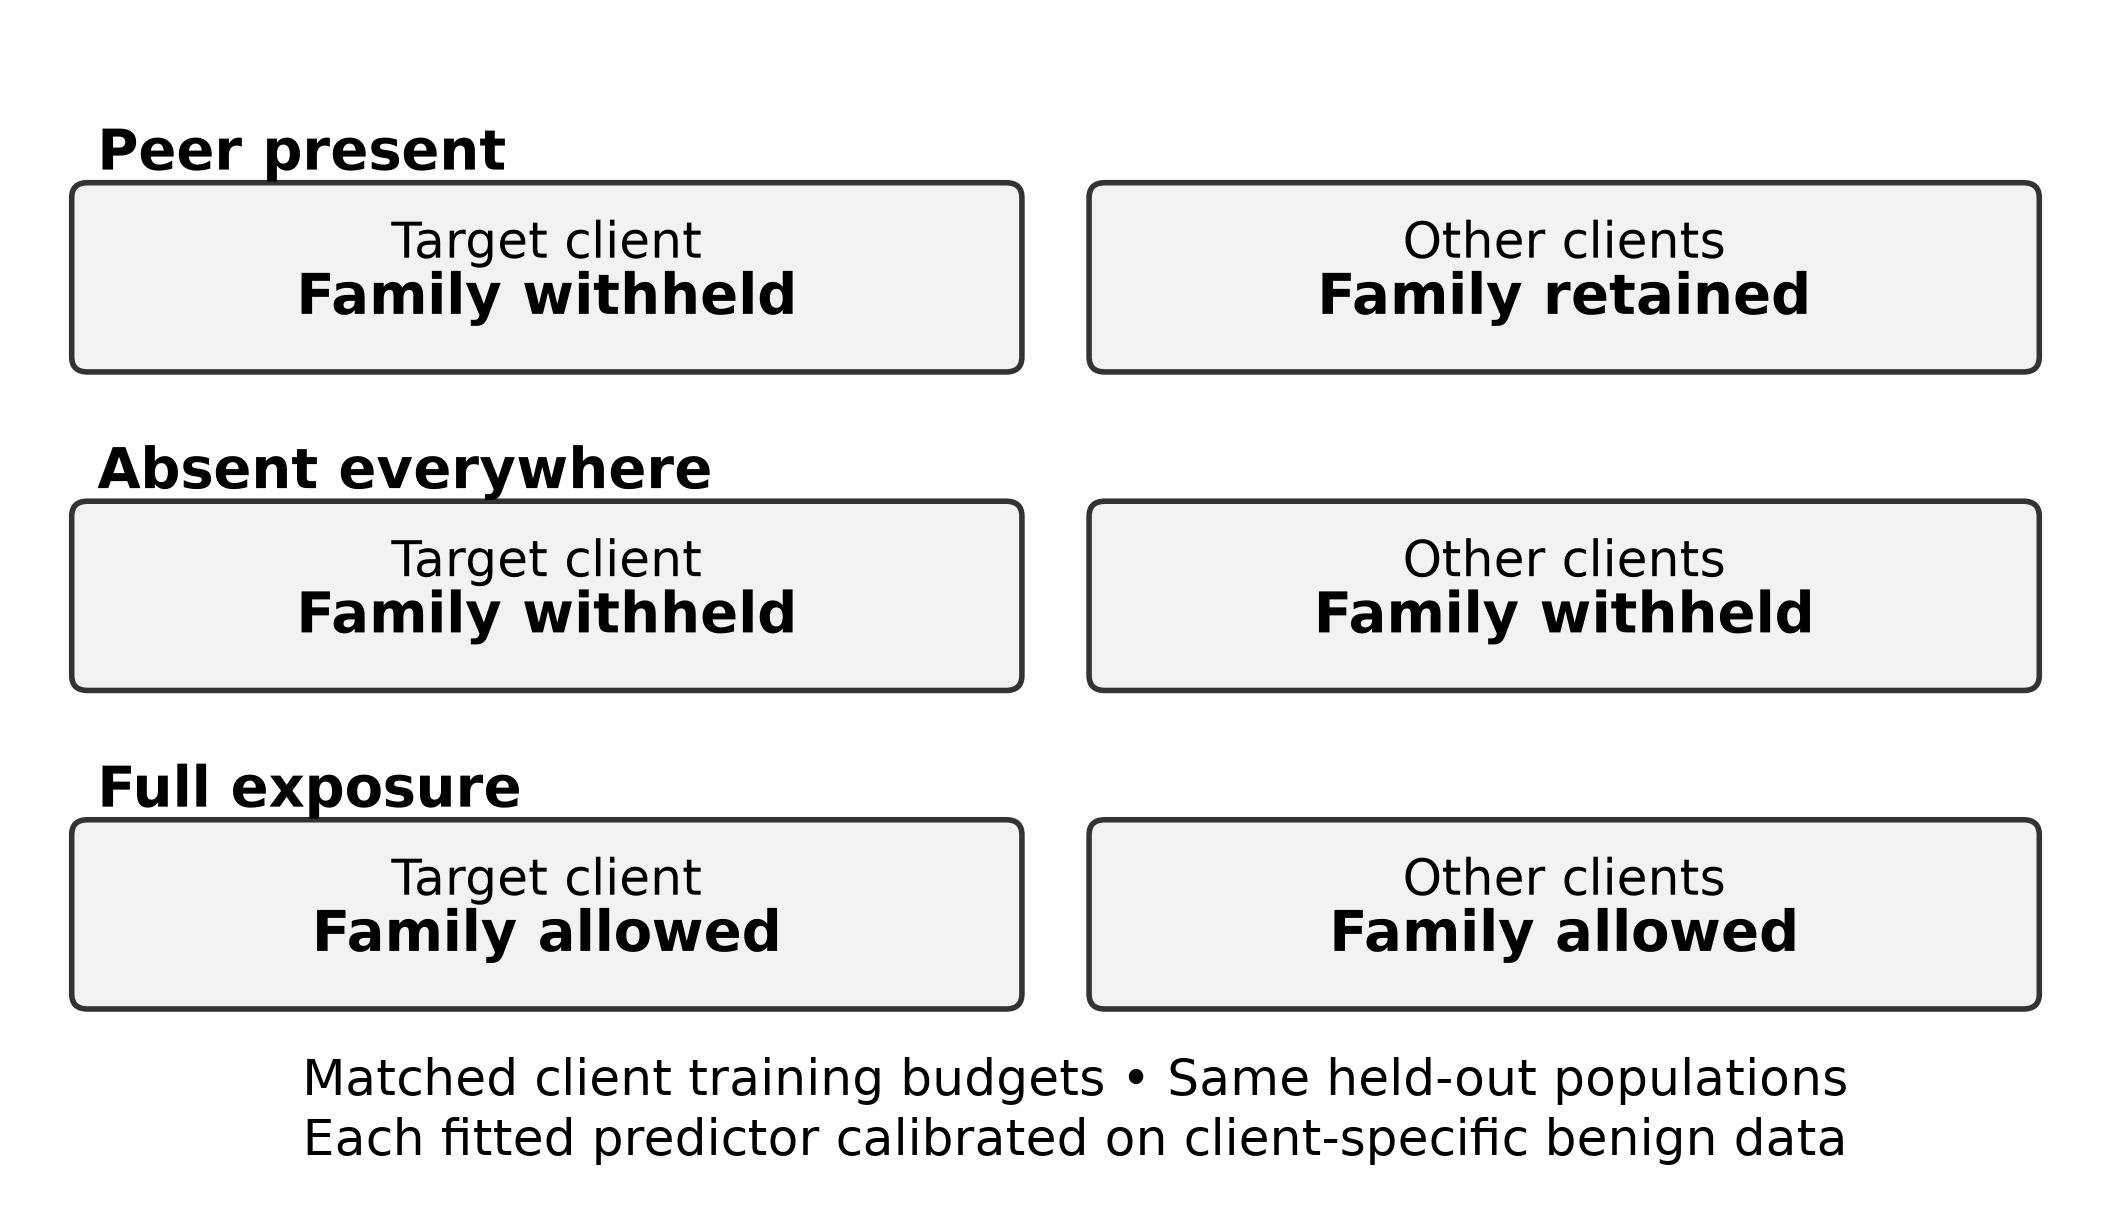
\includegraphics[width=\linewidth]{figures/Figure_1.png}
\notes{The schematic illustrates one target-family pair. Each run can assign several families to different targets. In the peer-present condition, a selected family is withheld only from its assigned target, which may retain other selected families. In the absent-everywhere condition, all selected families are withheld from every client. Replacement examples preserve the 6,000-sample training budget per client. Full exposure removes the deliberate exclusions but retains the budget.}
\end{figure}

Some obscurer families can appear in multiple runs for one target. As mentioned replacing them will keep the amount of client samples constant but alter the distribution of malware/benign programs. We also replace each arms fits with benign scores. So expect numbers to vary. The CTK comparison captures this distribution and recalibration effect of obscurer families. It will not represent what one family contributes.

Natural scarcity looks at families where their target accounts for less than 5\% of their federated fit. These must contain at least 150 example of peers fits and 15 examples on their test split. It doesn't null out the target family amount. There could be a few local training examples. This question tries to see if seeing examples of that family helps. Similar to above it will vary which target families are chosen and the definition of scarcity being used. Therefore we use it as a sensitivity not an equivalent measure.

Future work could expand on both the number and type of family. An exact dose would look at sets of 0 10 25 50 100 and 200 effective peer examples. Ensuring the target family is absent and measure what the actual support was. We could also create a placebo arm by choosing another family of malware and following similar principles of support matching and allocation. Both of these are subject to the families we choose and how much budget we have to allocate to replacements.

\subsection*{Aligned Representation Extension}

It intersects our retained LAMDA applications with each source we need from McNdroid by hashing application ids. This leaves 554,136 applications that consist of 170,256 malware and 383,880 benign applications. We have 925 static features from LAMDA 2,390 static features from McNdroid, 2,793 columns for call graph and 17,483 columns for the report-json file. These graphs are provided from McNdroid's ability to derive information from a graph. It is not some new graph model that we have built. Report will be transformed using sign log then we fit to each of the arms inputs as they are configured. This is comparing these forms of data not everything that can be done with McNdroid.

Every representation will keep their original labels and clients from the shared population of applications. We use the main representations and package to get the family names and filter them to only contain what we share. We can get a good set of comparisons with matching applications but we don't filter family matches for our other forms. We look at families we feel show interest in their response such as hiddad, gappusin and revmob. We also take leadbolt, airpush and dowgin as well as adwo to compare against. All of these families we want to see how they acted previously. So these are not true outside comparisons.

\section*{Learning and Evaluation Protocol}

\subsection*{Learners and Frozen Training}

Our base model was an MLP with 256 and 64 units in two hidden layers. Rectified linear activations were used along with a dropout probability of .1. Binary cross entropy on logits using an Adam optimizer, lr of .001 and batch size of 256 and no weight decay. Each local model was trained for 10 epochs on their clients budgeted fit sample. The global model was trained for 20 epochs on all four of the budgeted samples from the clients. This is just what we felt comfortable with as far as number of epochs and does not reflect each learner finding its optimal solution. We have summarized these parameters below in Table~\ref{tab:2} that will help to evaluate our results.

\begin{table}[!htbp]
\caption{Conditions of the Primary Controlled Study}\label{tab:2}
\small
\begin{tabularx}{\linewidth}{@{}l>{\raggedright\arraybackslash}X@{}}
\toprule
\textbf{Component} & \textbf{Setting} \\
\midrule
Source and representation & LAMDA var\_thresh\_0.01; 925 binary features \\
Partition & Package/feature connected components; 60/20/20 fit/calibration/test; best support among 16 attempts \\
Training volume & 6,000 fit rows per client; 1,500 in lower-support sensitivity \\
Primary eligibility & Target fit ≥20; peer fit ≥150; federation test ≥50; remaining target fit ≥500 \\
MLP and optimization & 256/64 hidden units; rectified linear activation; dropout 0.1; Adam; learning rate 0.001; batch 256 \\
Training schedule & Local 10 epochs; central 20; federated 20 rounds × 2 local epochs \\
Adaptation & FedProx μ = 0.1; fine-tuning 2 epochs; equal probability blend \\
Operating points & Nominal FPR 5\% primary; 1\% and 10\% sensitivity \\
Primary inference & Seeds 100–109; paired effects; 9,999 BCa resamples; exact Wilcoxon; Holm across three contrasts \\
\bottomrule
\end{tabularx}
\notes{Support requirements refer to pre-budget pools. Family-macro, own-domain, and worst-client summaries use distinct denominators. Hyperparameters and statistical procedures were frozen before confirmatory evaluation. The stored resolved configurations of all confirmatory runs match the frozen run-level protocol.}
\end{table}

We used 20 rounds of FedAvg with 2 local epochs and all 4 clients participating each round. They are initialized with the current global parameter estimates at the beginning of each round and then returned after being fitted to their respective samples to be aggregated by number of fit examples. All clients will have an equal weight as they all had 6,000 fit examples. When making the local training call we create a new optimizer with the Adam optimizer each time. No states are saved between rounds. FedProx is the same except with a proximal strength of .1. We fine tune the fit FedAvg model by 2 more local epochs on the local clients fit data. Blend is made by averaging the local and FedAvg predictions with equal weight. We calibrated each predictor using their respective clients benign calibration observations.

We also have centralized learn as a baseline. With our federated methods we are distributing the learning process to our testing clients. We can then fine tune those models to learn about target data they did not see the hold out family on and blend them together. We had a development set to vary our local epochs and fine tuning amount as well as proximal strength for FedProx. These methods were used to create our final settings instead of based on test accuracy. The various learner tradeoffs will be explored in the results section.

We created alternative model learners to compare with our methods. First was a linear model binary classifier. Second was a histogram gradient boosted tree learner with a max of 100 estimations and 6 levels. Our local and central learners were compared to this model to see if our comparison still stands when using a different model class. The linear model also included a FedAvg model to see if any benefit would occur when using our linear method.

Our other graph and reports were transformed with the arm chosen fit observations. Local models were transformed by their fit observations and shared learners by their fit observations. We also use our min positive percent of 1\% when finding columns for our report input. These observations were not used to transform. Keep in mind that we are using our providers features and reduced with primary LAMDA. We believe this is an ok benchmark to go off of when using our features but could not go so far as to estimate our entire feature process.

\subsection*{Calibration and Metric Definitions}

Threshold is taken to be the empirical (1 − alpha) quantile of the benign calibration scores for each client and arm. We take the larger quantile. Applications are considered positive if they are above this threshold. Alpha = .05 is our main focus with sensitivity analyses performed at .01 and .10. If we have less than 10 benign calibrations × alpha we will consider our calibration inadequate. Due to ties in scores and potentially differing populations between calibration and test data our achieved test FPR will vary around alpha. At the run level we will allow a ±2 percentage point difference in the FPR (client-macro) at our main operating point. This is not a guarantee that each individual clients FPR will be within 2 points of each other. There is also no guarantee that having sufficient calibration support will satisfy this run level check.

Own-domain unseen-family recall is the percent of test applications flagged that are from the families we hid from each client. Only test applications from that domain are considered. The rates are averaged across clients who meet the threshold for own domain support. Federation-wide unseen family recall looks at the target clients detector on its hidden families from all four domains. Then the rates are averaged across the target clients. You could be testing the detector on applications that aren't from its corresponding market/era. There is more support to answer this question but the test population does not reflect what the client would normally see.

Family-macro unseen recall takes the mean recall of all target families we consider eligible on the federation wide test population. All entries are given equal weight. This is different than pooling hits for the hidden families on each client and taking the mean. Pooled micro recall is the pooled number of hits divided by the number of trials. Families with higher support are given more weight. For our confirmatory comparison we report the original client-macro estimand. However we specify our estimand of family macro in the dose response and family summary plots. Because some families may be higher responders than others or clients with higher responders our estimates may differ by choice in weighting.

We report nonhidden-malware (known-family recall) recall as well. This is the client macro mean recall on the test population for applications that are not part of our hidden families for that client. These may contain malware without a target family. We do not know if all family labels were seen during training. Achieved FPR is the mean of clients FPR on their benign test set. Worst client FPR is the largest client FPR. Worst client unseen recall will be the smallest federation-wide hidden family recall across the target clients per seed. Worst client can vary between arms so comparing differences in worst client is not directly saying that one client improved more than another.

Area under ROC and average precision are also calculated on the client level for all test applications on that domain. Averaged equally across clients. Using sklearns implementation of average\_precision\_score we label this AUPRC. This weights the precision at every increase in recall. Unlike a ROC which trapezoid the PR curve. Also dependent on test population proportion of classes. These are not limited to our hidden families at our operating point. When comparing them to unseen-family recall they are both on different test sets.

\subsection*{Statistical Inference and Evidence Status}

We have the original seeds from 100–109. For each pair we can calculate differences between arms using the same partition and targets. Summary statistics for the means, median, number of positive seeds and standardized effect sizes are reported. To get a confidence interval on the difference we use the 9,999 bootstraps on seed differences to produce our 95\% CI using BCa bootstrap. There are no zero or tied absolute ranked values among the 3 main comparisons so we can apply an exact Wilcoxon signed rank test with two sided \textit{p}-values. This will test if there is any symmetry about zero in the differences. Not testing if there is a difference from zero for the mean. We control for type I error using Holm correction across the 3 comparisons for the FedAvg federated wide breakdowns (Holm, 1979) with an alpha of 0.05. This correction only applies to the 3 comparisons and not to any other learners, population or family breakdowns. As well as later diagnostics.

A significance level was not the intent when choosing our practical value for CTK to be 3 percentage points and 2 points lower for nonhidden-malware. These are cut offs and should not be compared to a significance level that is testing for zero. Bootstrapping BCa means and signed rank tests test for different things and if they do not line up you should not change your method. By taking a bootstrap of components over withheld values we can assess if the test being applied plays a role in these estimates. These values would not provide a confidence interval on our seeds used to train the models.

By using four types of evidence we can assess what information is available. We define type A as our original confirmed evidence. Type B are any prespecified evidence that could add robustness or provide more information to our results (ex: sensitivity). Any evidence collected after confirmation that we use our previously saved data on we can label as Type C. Lastly if we decide to freeze another type of prospective work we can label it Type D and use future diagnostic as well but make sure to note which ones they are. Using seed values from 200–209 for our permutation extension, 300–309 for the extension that increases our family size, 310–319 for our exact dosing, 320–329 for our placebo/aggregation testing and 330–339 for our representation work. These all are not combined with our original seed values to create confirmatory evidence. If we were to combine our original families with our extended replication families in one seed we would only have a sample of 10.

The GitHub link provided will include all the information to create and evaluate our model. This will also include our source code, configs, data outputted and fingerprinting information: \url{https://github.com/naslouby-salahe/ctk-android}. Our package of evidence will include our run revision f6302f7906824945731dadbbeb44357f3d025aaf and all revisions that correspond with our analysis with a clear path to analysis. All of our results came from our final deterministic run once we enabled gpu dropouts seeding and determinism for our kernels. We ran our model two times before our final run with these confirmatory settings that did not give us reproducible results bit for bit. These runs gave us a FedAvg CTK score of \textasciitilde{}11.7 points. We will not pool these values with our final run for reporting purposes. Fingerprinting of source data along with our manifest will allow us to point to what values we used and what our output was. Data will need to be obtained externally as well as a device capable of running our model to train. We will have seeds that can help assess how much variance our results could give given the corpus we have chosen.

\section*{Experimental Results}

\subsection*{Primary Controlled-Exposure Results}

As confirmed with the comparison above we can say there is a significant amount of benefit from complementary peer exposure. With the families selected not existing on any clients the FedAvg federation wide unseen family recall goes from 52.41\% to 64.36\% when our peers have them. Locally this number is 50.90\% and when all clients have these families FedAvg gets a 67.64\% recall. Our mean FPR achieved is 5.04\% for no where they exist 5.09\% with peer exposure and 5.04\% when they are on every client. Due to the comparable means we can say these comparisons are at the same FPR rate. We hide client variation when looking at the mean FPR. Mean worst client FPR is 6.60\% with peers having them and we see a max worst client FPR of 9.89\% over our 10 seeds. Table~\ref{tab:3} shows this effect along with error estimates in Figure~\ref{fig:2}.

\begin{table}[!htbp]
\caption{Primary Paired FedAvg Decomposition at Nominal 5\% FPR}\label{tab:3}
\small
\begin{tabular*}{\linewidth}{@{\extracolsep{\fill}}lcccc@{}}
\toprule
\textbf{Contrast} & \textbf{Mean (pp)} & \textbf{95\% BCa CI (pp)} & \textbf{Holm \textit{p}} & \textbf{Positive seeds} \\
\midrule
CTK & +11.96 & [+9.15, +15.21] & 0.00586 & 10/10 \\
Pooling & +1.51 & [−4.15, +6.10] & 0.32227 & 7/10 \\
Total & +13.46 & [+8.82, +17.04] & 0.00586 & 10/10 \\
\bottomrule
\end{tabular*}
\notes{Ten confirmatory seeds, 100–109. CTK = peer present − absent everywhere; pooling = absent everywhere − local; total = peer present − local. Realized FPR: local 4.99\%, absent 5.04\%, peer 5.09\%, full exposure 5.04\%. Intervals summarize seed-paired mean differences; \textit{p} values are exact two-sided signed-rank results adjusted across these three contrasts. pp = percentage points.}
\end{table}

\begin{figure}[!htbp]
\caption{Complementary Exposure and Generic Pooling in the Primary FedAvg Comparison}\label{fig:2}
\centering
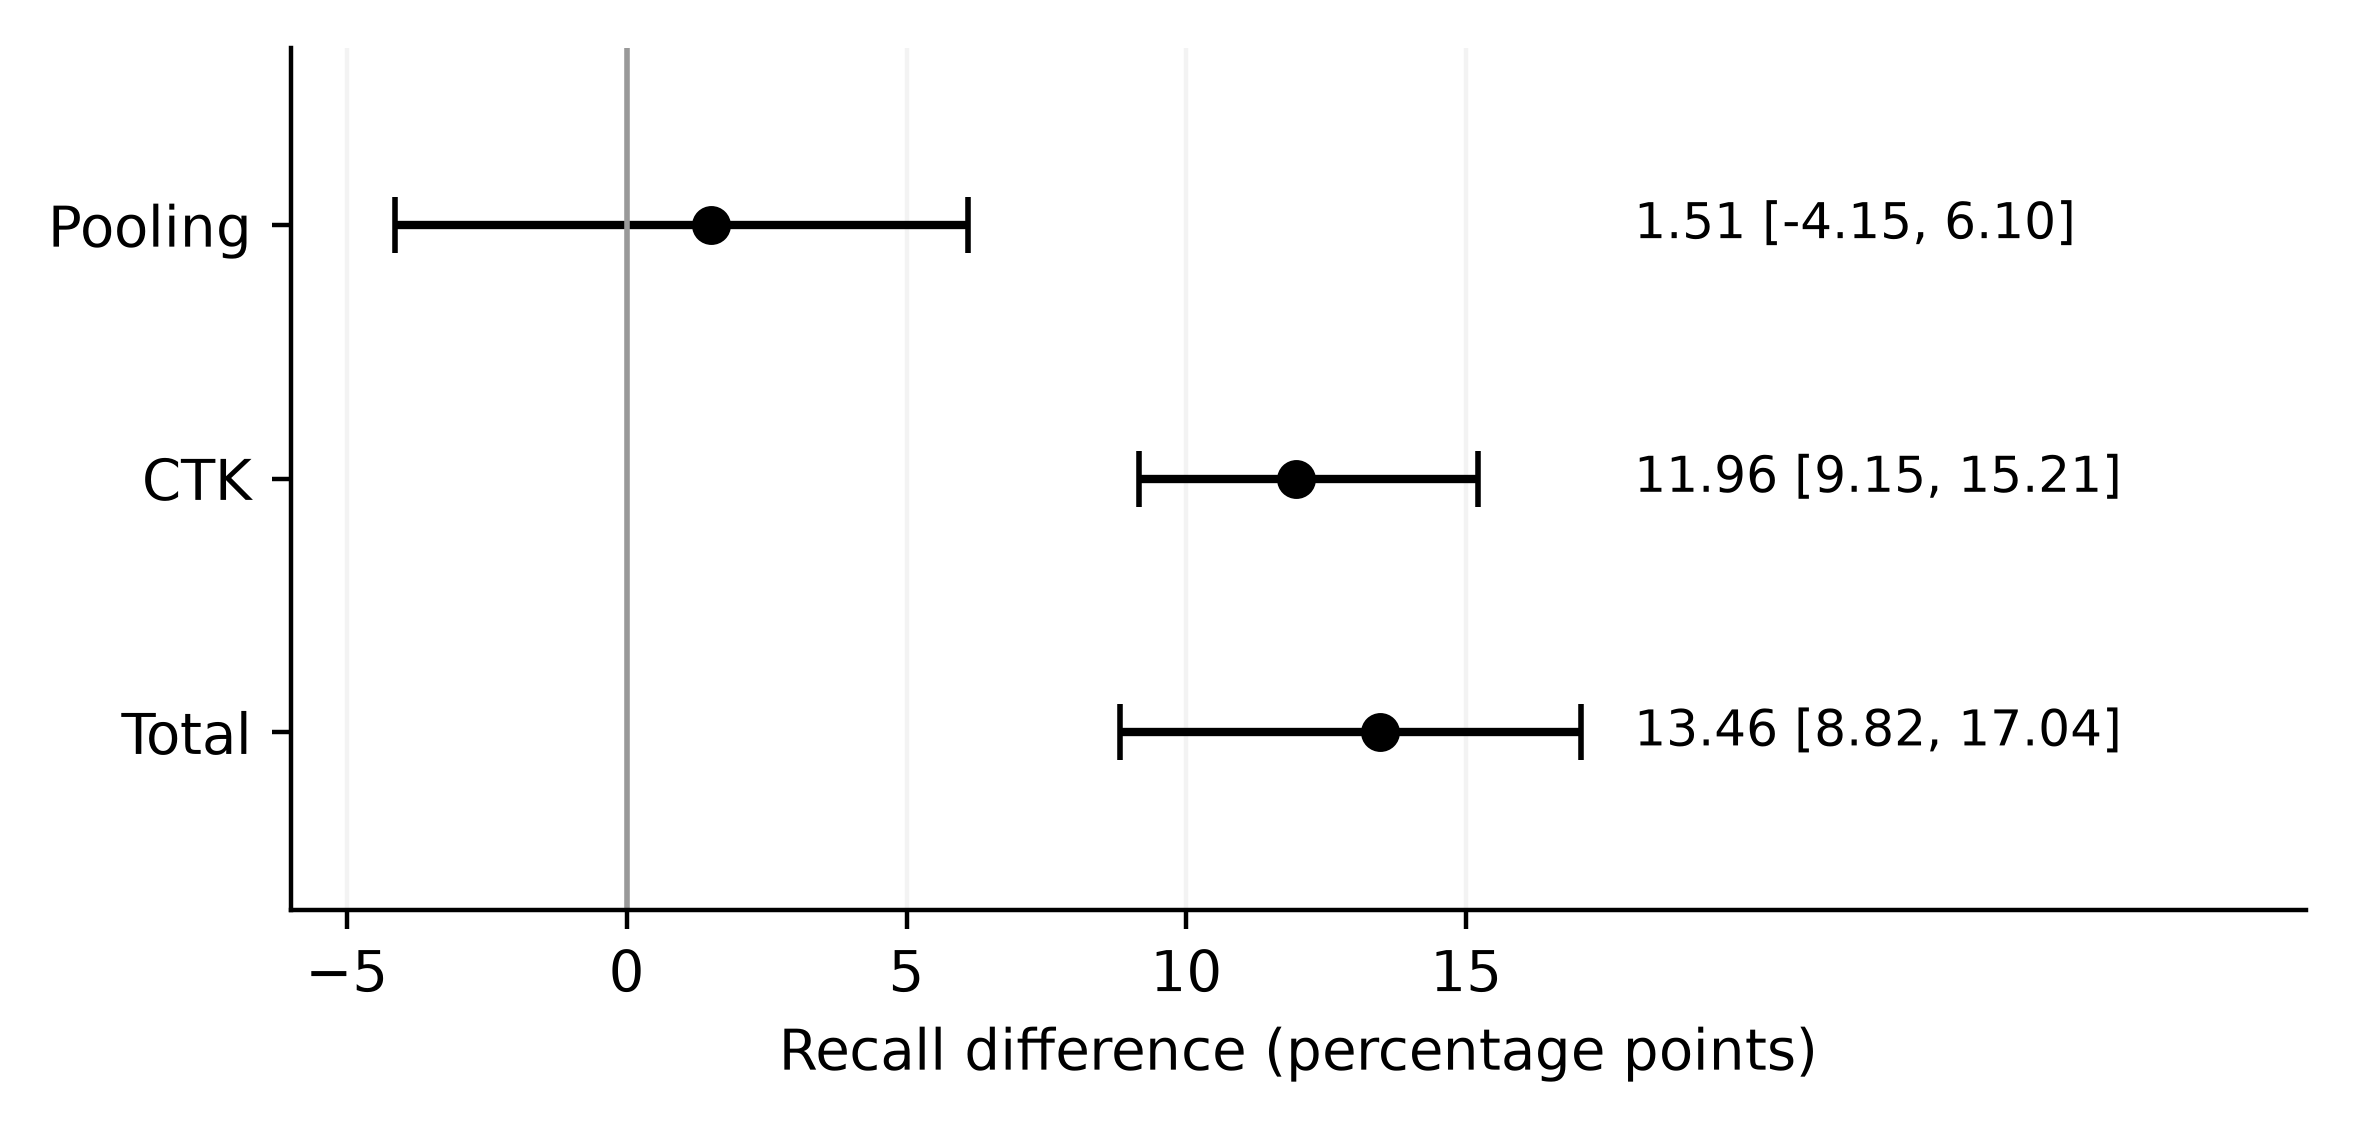
\includegraphics[width=\linewidth]{figures/Figure_2.png}
\notes{Point estimates and 95\% BCa intervals in percentage points. Federation-wide client-macro unseen recall, nominal 5\% FPR, seeds 100–109.}
\end{figure}

As shown by Table~\ref{tab:3} and Figure~\ref{fig:2}, we see that the CTK effect and total gain are positive for all 10 seeds in the confirmation. The residual collaboration effect is consistent with a small negative or positive effect. Notice that our estimates of CTK and pooling add up to 13.47 due to rounding, they add up to the total of 13.46 when not rounded. Our definition of CTK accounts for the difference in training compositions shown in Figure~\ref{fig:1}. On average there are 2,073 samples that are different between peer-present and absent everywhere out of 24k fitted samples.

Studies testing if our effect requires knowing families are covered below. These include family permutations, wrong family placebos and exact dose studies. Original seeds and new seed evidence will be shown separately for these results.

Using our main pooled estimate we find peer present to have a 66.07\% federation wide recall rate. Absent everywhere has a 52.97\% recall rate and fully exposed clients have a recall rate of 70.19\%. Because the central learner and federated learner train for different numbers of rounds we cannot say that one is better than the other in these settings. Using our procedure of training the peer present case will result in lower recall rates than that of the fully exposed mean. As discussed before there is an upper bound for how much you can be exposed to. Different families and seeds may produce different orderings.

FedAvg results on own domain unseen malware show a recall improvement of 10.85 points over training with absent everywhere (6.97–15.25). Residual collaboration is −7.60 points (−11.81, −4.03) resulting in a total improvement of 3.26 points (1.26, 5.63) over local learning. A significant portion of our complementary exposure effect comes from the decrease seen in the absent everywhere case. Recall that we showed an 11.96 point effect for our measure of CTK when using federation wide hidden family testing malware. Comparing peer present against absent everywhere and comparing peer present to local learning with own domain hidden family testing malware yielded a 3.26 point improvement. We note that these own domain results are of the secondary populations and are not Holm adjusted.

When looking at the family macro level we find our CTK effect to be 12.44 (10.09–15.55) and a total gain of 10.57 points. Our client level metric of worst-client shows our CTK effect to be 18.49 (13.88–26.29) and a total gain of 14.88 points. When each hidden family test application is weighted equally our CTK effect is lower. But still positive for all 10 confirmation seeds at 6.58 points (4.64–8.65). Our pooling gain was 4.00 points with a total gain of 10.58 points. Much of the discrepancy from our client macro result comes from the client dowgin. Dowgin makes up about 47\% of our hidden family test applications and does not have a significant CTK effect. Removing dowgin results in a micro-pooled CTK effect of 12.24 points. These tests use different ways of aggregating so keep that in mind. When comparing the worst client we are comparing the minimum for each arm. So it is not saying that the one client that is the worst improved by this amount. When looking at FedAvg we see positive CTK effects when looking at federation wide recall at both alternative operating points. At 1\% FPR nominal we have an effect size of 7.85 points and 13.78 points at 10\%. With our original operating point of 5\% we found an effect size of 11.96 points. We see varying degrees of our exposure effect at different operating points.

\subsection*{Learning-Strategy Comparisons}

There are six alternatives with peer present that are displayed in Table~\ref{tab:4}. A .19 point (−1.12, 2.94) difference between FedProx-minus-FedAvg post confirmatory federation wide unseen recall was observed. Not enough to determine if one is superior. For every alternative learner there were all ten seeds showing complementarity. On average centralized training showed 13.10 points of CTK. FedProx showed 13.20 points and fine-tuned FedAvg showed 8.20 points with blending showing 7.60 points. Depending on which learner you use you will get more or less CTK but never negative. Centralized learning produced the highest descriptively federation wide mean with. Using different methods of training and sharing information.

\begin{table}[!htbp]
\caption{Peer-Present Learner Performance at Nominal 5\% FPR}\label{tab:4}
\small
\begin{tabular*}{\linewidth}{@{\extracolsep{\fill}}lccccc@{}}
\toprule
\textbf{Learner} & \textbf{\makecell{Federation\\unseen}} & \textbf{\makecell{Own-domain\\unseen}} & \textbf{Worst client} & \textbf{Nonhidden} & \textbf{FPR} \\
\midrule
Local & 50.90 & 50.67 & 28.92 & 73.06 & 4.99 \\
Central & 66.07 & 56.27 & 41.42 & 72.92 & 5.10 \\
FedAvg & 64.36 & 53.93 & 43.79 & 69.46 & 5.09 \\
FedProx & 64.55 & 55.98 & 37.90 & 72.13 & 5.09 \\
Fine-tuned FedAvg & 62.16 & 51.64 & 40.35 & 69.33 & 5.03 \\
Blend & 63.66 & 57.21 & 37.63 & 74.77 & 5.12 \\
\bottomrule
\end{tabular*}
\notes{All entries are percentages averaged over ten confirmatory seeds. Worst client is the within-seed minimum federation-wide unseen recall. Other recall and FPR columns follow the macro definitions in the protocol. Arm rankings are descriptive; table levels are not confidence intervals or adjusted pairwise superiority tests.}
\end{table}

Recall on the nonhidden-malware task will affect this rank as well. FedAvg decreased 3.61 (CI −4.50, −2.85) from local learning and fine-tuned FedAvg decreased 3.74 (−5.31, −2.82). Both of these averages are greater than our frozen value of 2. FedProx was off by 0.93 and central learning only 0.14. Blend increased by 1.70. Using our metric for tolerance allows us to compare averages with a set amount. This isn't saying they are equivalent with an interval or for all clients.

Similar to Figure~\ref{fig:3} we can see that average and min recall differ. FedAvg had the largest descriptive average when using the minimum for each seed. Despite having a larger decrease in the nonhidden-malware task. FedProx and Blend both kept more recall for the nonhidden-malware task but their minimums were smaller. This shows that there are many things to consider when picking which learner to use. How much you are willing to lose and what your testing will consist of.

\begin{figure}[!htbp]
\caption{Mean and Worst-Client Unseen Recall Across Learners}\label{fig:3}
\centering
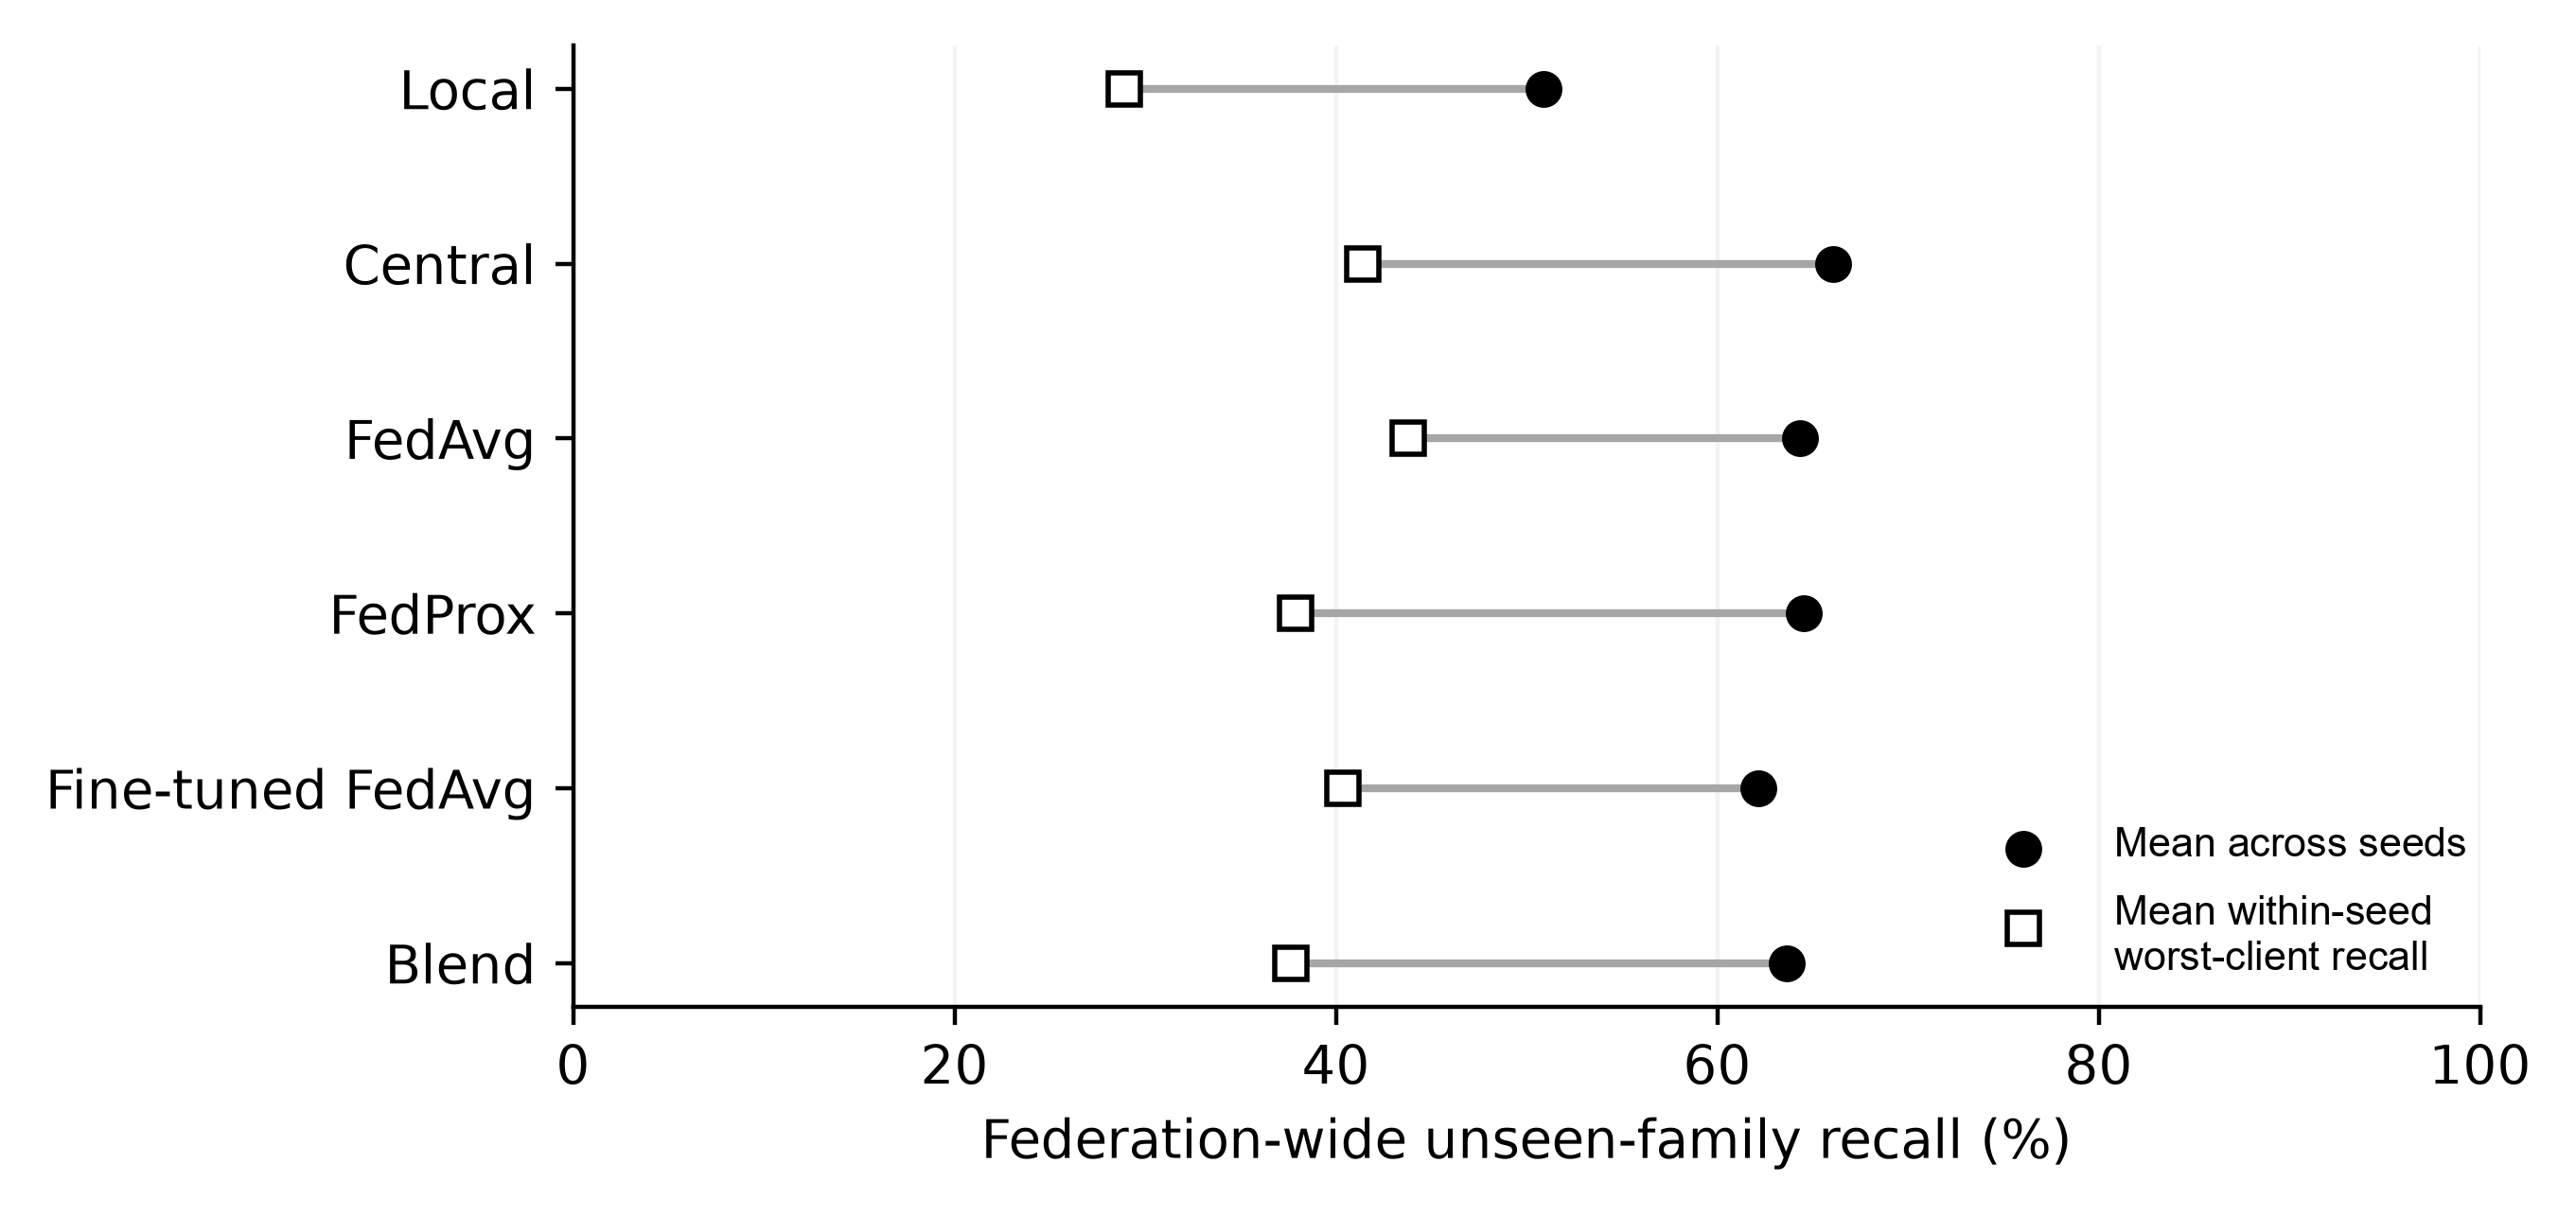
\includegraphics[width=\linewidth]{figures/Figure_3.png}
\notes{Peer-present condition, nominal 5\% FPR, seeds 100–109. Points show means across seeds; no uncertainty interval is implied. Worst-client identity can change across arms.}
\end{figure}

While coverage for hidden-families increased we saw an overall decrease in discrimination. After applying confirmatory results from FedAvg-minus-local we have −0.01166 change in mean AUROC and −0.02011 change in mean average precision. This shows for all thresholds on our entire own domain test set. The previous result is on select families that were hidden so both are important when evaluating a detector.

\subsection*{Malware-Family and Client Heterogeneity}

As seen in Figure~\ref{fig:4} when we look at Primary-family recall between our different exposures. The best two conditions were revmob and leadbolt both gaining 33.38 and 27.75 points on average respectively. When compared to local learning we can see that there is a significant gain from exposure. However revmob is still not meeting a 60\% recall rate when fully exposed using FedAvg. Which shows you can gain a lot from exposure but may not be enough.

\begin{figure}[!htbp]
\caption{Family-Specific Recall Across Exposure Conditions}\label{fig:4}
\centering
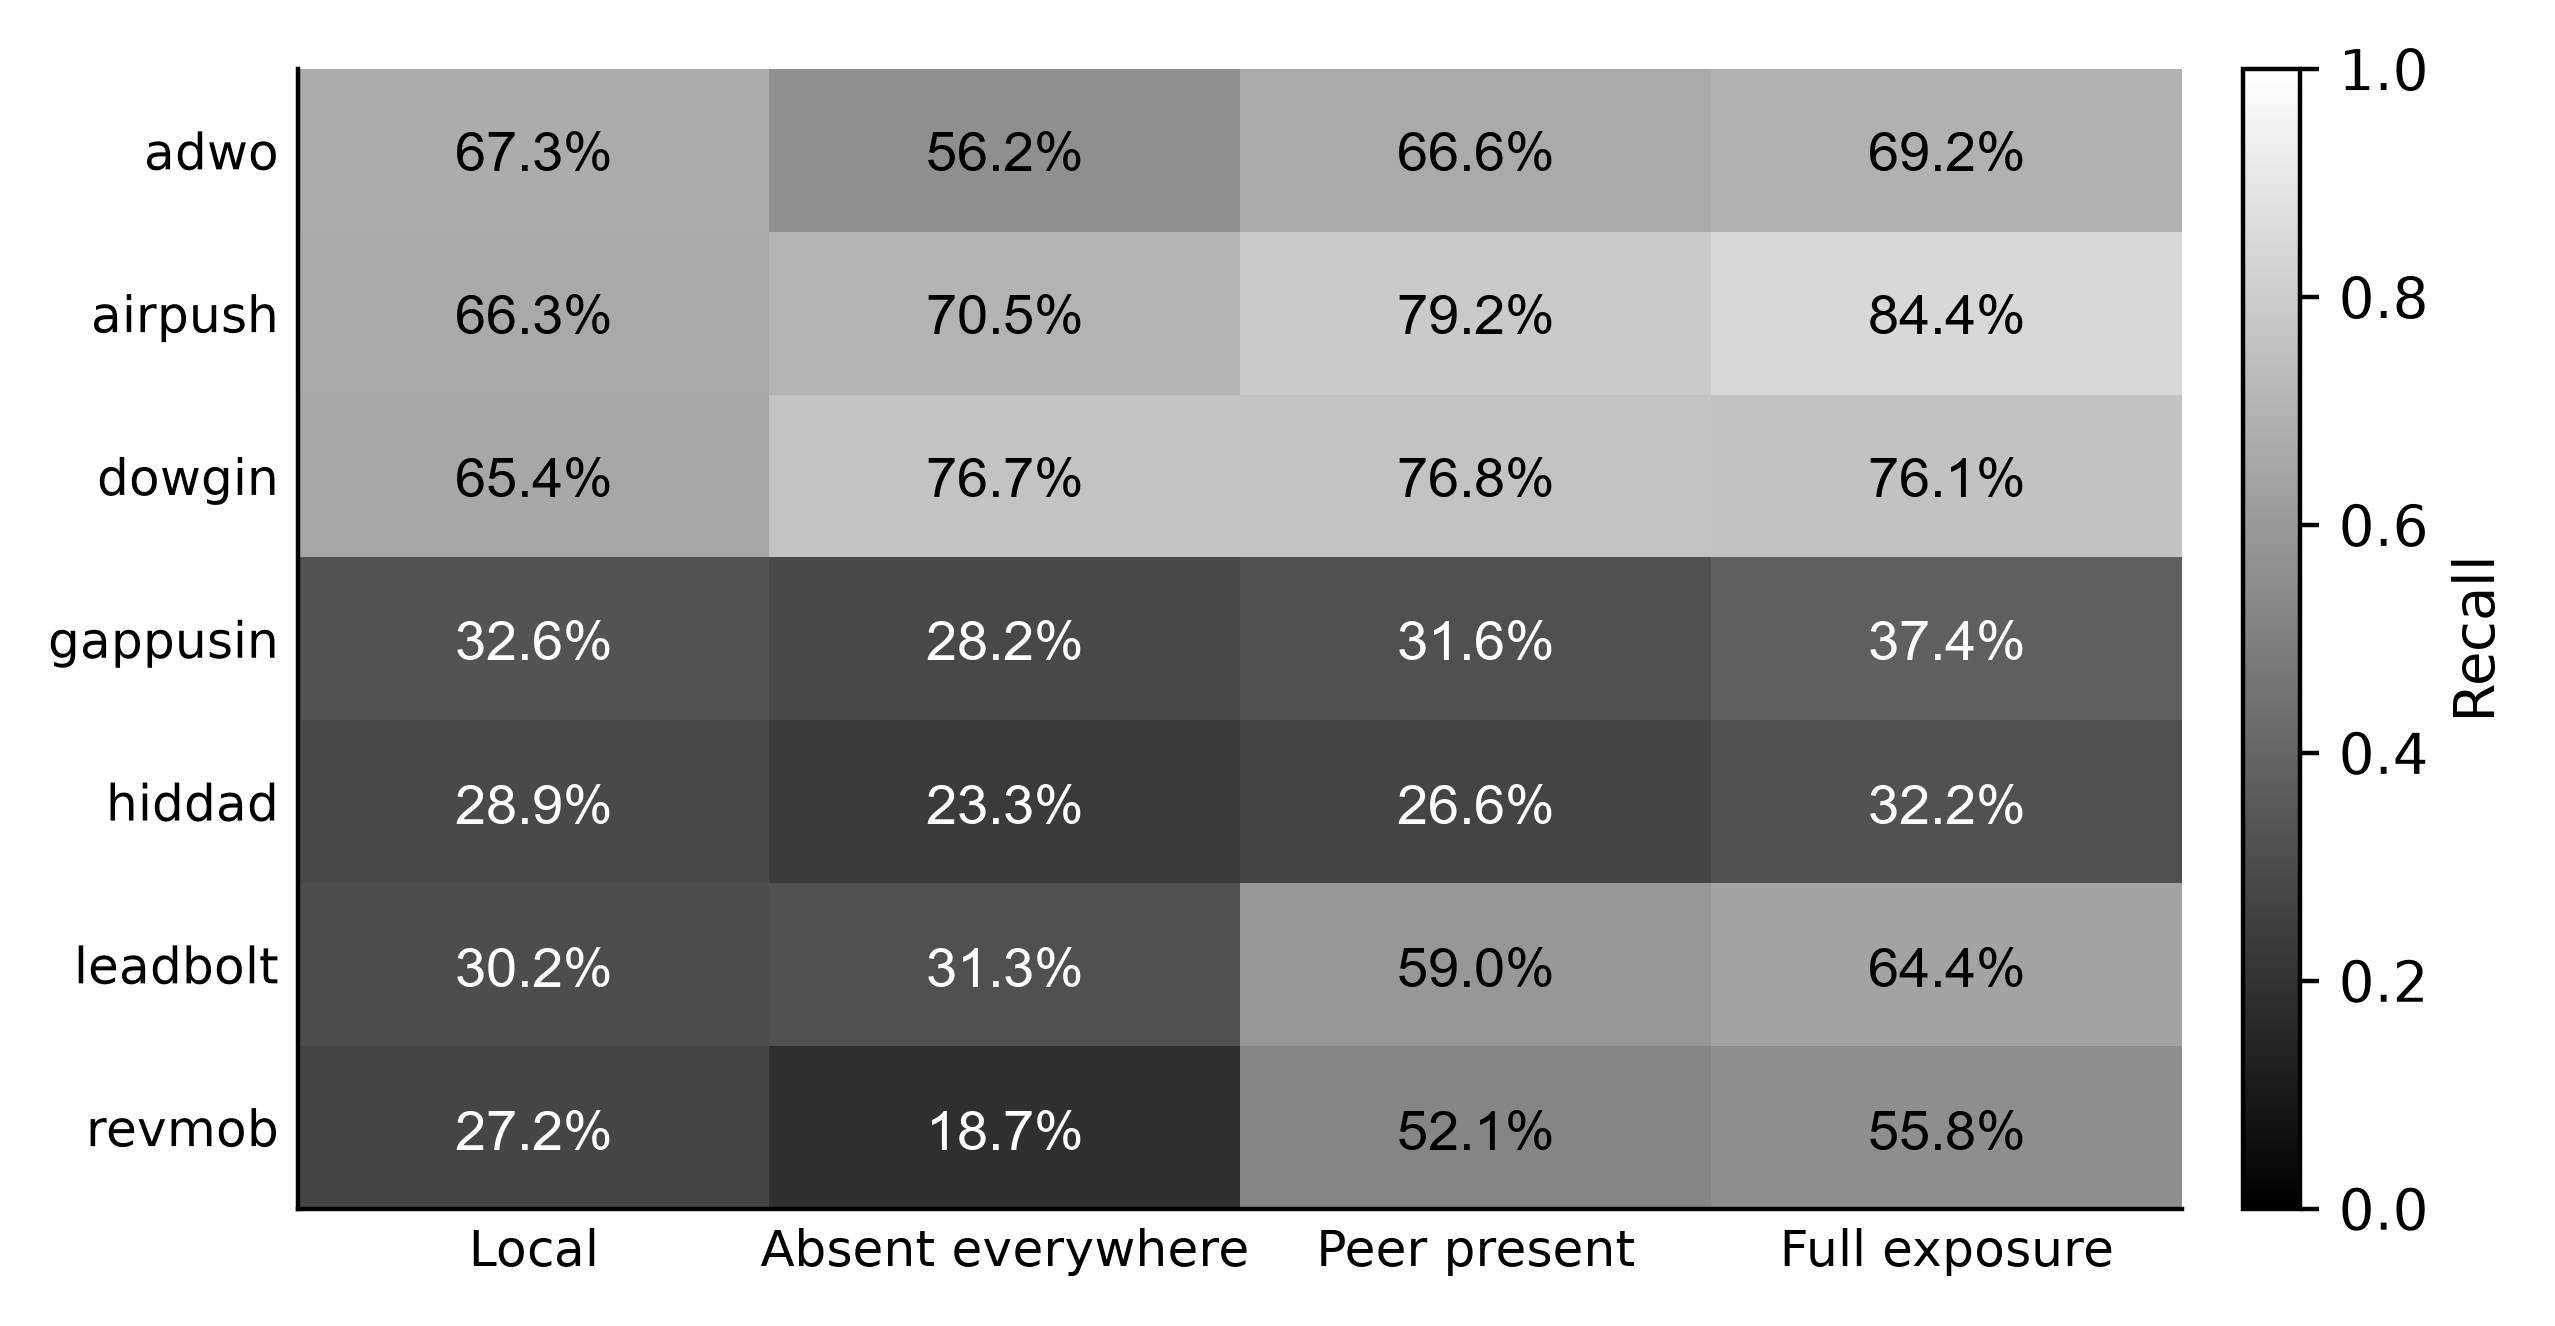
\includegraphics[width=\linewidth]{figures/Figure_4.png}
\notes{Cells show mean recall percentages to one decimal place at nominal 5\% FPR across seeds 100–109. Full exposure refers to FedAvg and is a finite reference. The grayscale bar expresses the same recall values as proportions.}
\end{figure}

Dowgin has more of a gain from pool: with a large local vs. collaborative increase its CTK was just 0.14 points. Adwo can be said to have repair from negative transfer: their CTK was a large 10.37 points that almost completely made up for the lack of everywhere. Peer-present is still less than local though. These differences can be seen when looking at their respective plot values. Not grouping both into the success of complementing each other's exposure.

Gappusin and hiddad show some response to the static representation. With a mean CTK of 3.46 points and 3.25 points. But have peer-present recalls of only 31.63\% and 26.57\%. Which both are below their local mean recall. When shown their full amount of exposure their center recalls were still at 42.38\% for gappusin and 28.68\% for hiddad. So this leads me to ask about their representation instead of saying they will increase when exposed more than locally. Airpush is in between with a CTK of 8.71 points and a peer-present of 79.24\%. We have to keep in mind that our family estimates for the primary family are an overview of our chosen targets with frozen seeds.

There are decreases when looking at replicating: dnotua had a mean of −8.24 points for CTK and zdtad at −2.06 points. Inmobi and domob both had positives of 13.63 points and 12.04 points. There are also only six seeds instead of ten for utchi and zdtad. Our replicated aggregate result was positive with some families decreasing CTK and having lower standard deviation. So we cannot say all names would increase if given the proper exposure.

The following are breakdowns by client which would place them under class C. The federations avg CTK using FedAvg was 8.35 points at Anzhi, 7.58 at AppChina, 9.18 points at play-early and 32.03 points at play-late. These all have different numbers of seeds that contribute to their total. 8 seeds for anzhi, 10 for appchina, 10 for play-early and 6 for play-late. Which leads to play-late having such a high average because of those constraints. Anzhi also increases a small amount at 1.34 points even with it having a positive CTK. When diagnosing client levels it decreases by 6.93 points for nonhidden malware. Its own domain total also varies great between clients at −2.80 points for anzhi, −0.40 appchina, 6.48 play-early and 13.61 play-late. Again having standard deviations that cross 0 for the first two. Which shows our aggregate of increasing on own domain is not constant across all four clients. Play-late would also only have around 107 test applications that are hidden per seed. Which would lead us to believe it could be due to their market as well.

\subsection*{Peer Exposure and Dose Response}

Requested peer cap amounts were very different than actual fit exposure. With peer caps of 100 and 1,000 the mean effective dose for FedAvg was 9.03 and 79.39 since peers were sampled with budgets after being capped. All available had an average of 296.19 examples and family-macro CTK of 12.44 points. Only all available exceeded 100 fitted peer examples on average for each family. So when requesting a peer cap we can expect higher exposure than what is actually used.

When specifically setting how many peers to fit we can see that across all primary and replication families the family-macro federation wide CTK for FedAvg is 2.92, 4.90, 7.83, 12.48 and 14.49 points with 10, 25, 50, 100 and 200 peer examples. These averages are plotted in Figure~\ref{fig:5} with 95\% BCa CIs. There is always a positive effect for all 10 seeds of extensions. With 10 peer examples the interval is between 2.31 and 3.64 which contains our cutoff for 3 points being useful. And at 25 the interval is 3.87–5.89. Positive effect may not be large enough to reach cutoff.

\begin{figure}[!htbp]
\caption{Exact Peer Dose and Complementary Gain}\label{fig:5}
\centering
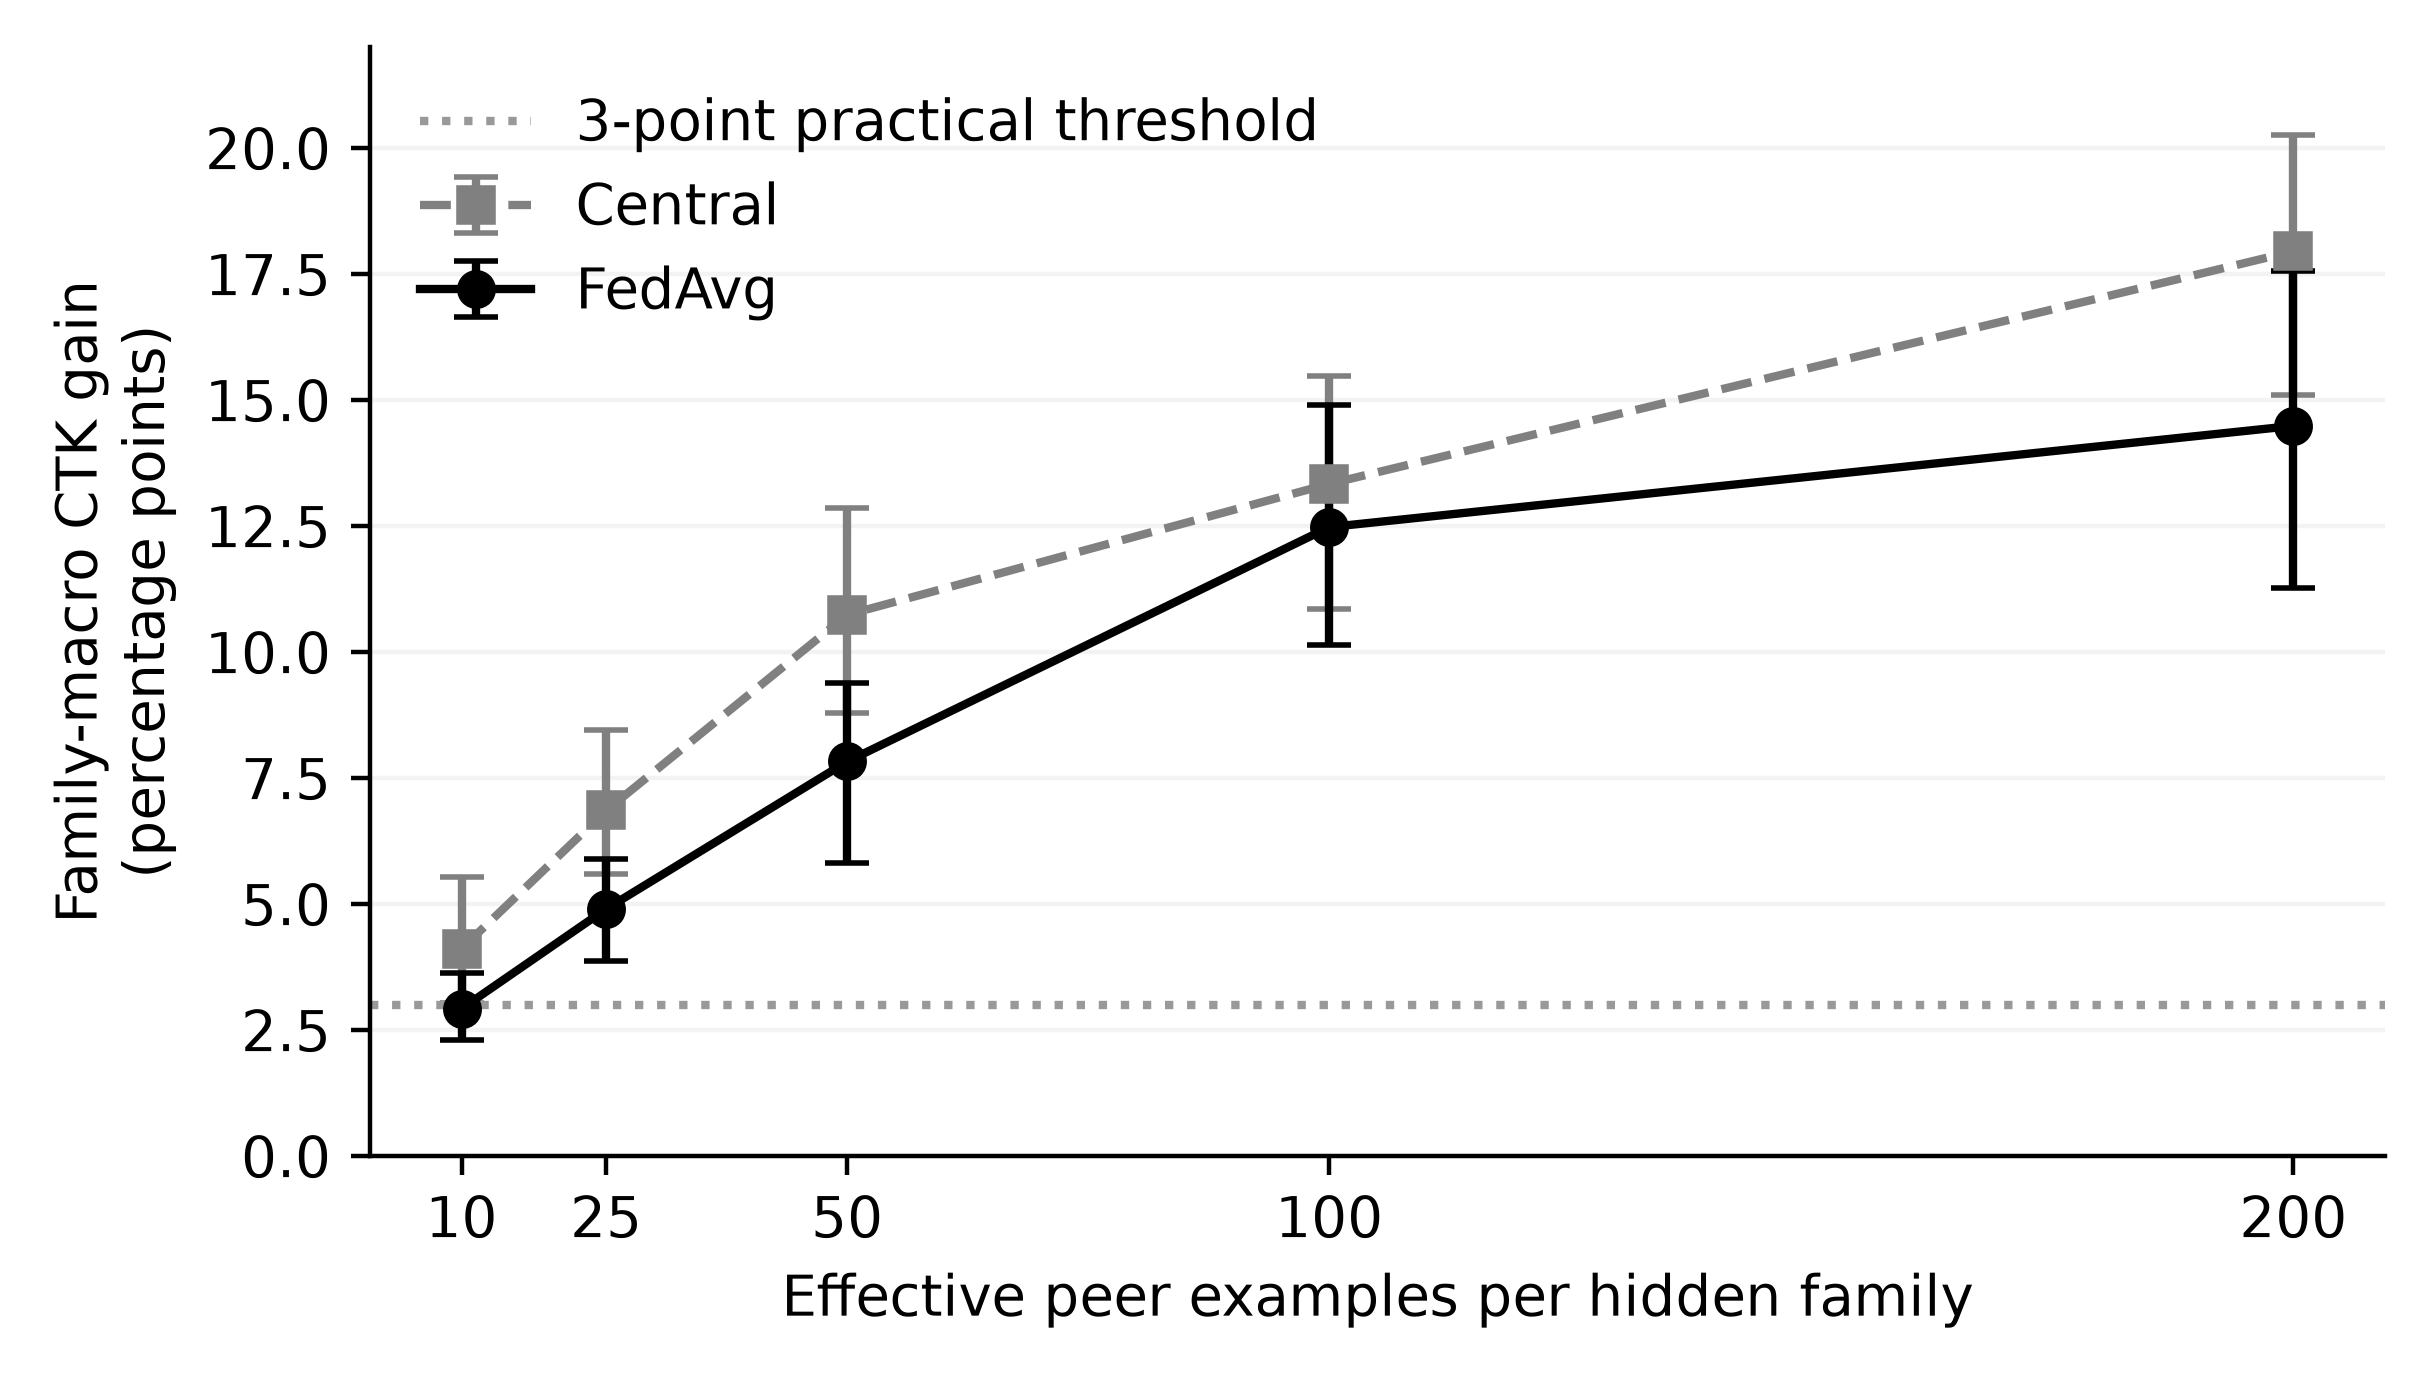
\includegraphics[width=\linewidth]{figures/Figure_5.png}
\notes{Prospective extension, seeds 310–319. Family-macro federation-wide effects pooled within seed across primary and replication sets at nominal 5\% FPR; 95\% BCa intervals. The dotted line marks a practical threshold, not a universal dose requirement.}
\end{figure}

Mean curves go up. Though there is no specific value that can be identified as saturating from the last increase. Increase from 100 to 200 was 2.01 (interval −0.06 to 4.06). And the increase from 50 to 100 was 4.65 (interval 2.43 to 7.09). Pooled increase would be all family sets combined. From 100 to 200 example of peers there is an increase of 4.23 points (interval 2.53 to 6.55) for the primary set. Only .03 (−3.91 to 2.54) points for the replication set. So for the primary set it continues to increase over the given ranges. However for the replication set the mean stays roughly the same. There is no indication of a shared satting point or minimum dosing level. As shown with different families having different doses. Dowgin can stay close to zero or slightly less than zero even at the high end of dosing. With our frozen consistency the 0 dose arm and none everywhere have the same observed effect.

\subsection*{Negative Controls, Replication, and Robustness}

Family-permutation control breaks alignment of families to applications while preserving whether an app is malicious or not. Original FedAvg federation wide CTK of 0.30 points with a CI of −0.36 to 1.02 at a nominal FPR of 5\%. This is considered resolved using the ±3 points equivalence criteria. Original own domain CI was larger extending up to 3.04 points which is still not resolved. Extension federation wide CTK was −0.21 points and own domain CTK was −0.07 both are within our ±3 point threshold. With additional seeds we further demonstrate that our controls hold however original own domain was still not resolved.

Table~\ref{tab:5} shows our wrong family placebo as well as our CTK minus placebo. We see a positive effect for CTK minus placebo across all ten extension seeds. If we pick another family with enough support we are unable to duplicate this effect from the chosen family. Since we cannot find an equivalent support that can account for all the properties when reallocating to other peers we know this control helps show specificity when replacing with families.

Using Table~\ref{tab:5} we found 8 out of the seeds to be positive using disjoint families. With a mean CTK of 5.08 points we can say that is practically significant. However the CI does not reach that amount. Using linear FedAvg, central tree and with less train support all showed positive CTK. We also changed our family support to be low and high as well as using only packages showed positive CTK. We also tried changing the partition salt to three other options all gave a positive mean CTK. These experiments show more cases within the same corpus and construction that our method finds a positive effect.

\begin{table}[!htbp]
\caption{Selected Replication, Sensitivity, and Control Effects}\label{tab:5}
\small
\begin{tabular*}{\linewidth}{@{\extracolsep{\fill}}lccc@{}}
\toprule
\textbf{Comparison} & \textbf{Class} & \textbf{Mean (pp)} & \textbf{95\% BCa CI (pp)} \\
\midrule
Disjoint family set & A & +5.08 & [+2.28, +7.10] \\
Natural scarcity & B & +11.19 & [+9.46, +12.59] \\
Linear FedAvg & B & +9.37 & [+7.54, +10.97] \\
Centralized trees & B & +10.18 & [+7.59, +13.70] \\
Lower training support & B & +10.99 & [+8.71, +13.52] \\
Lower family support & B & +14.01 & [+11.46, +16.22] \\
Higher family support & B & +11.59 & [+9.17, +13.75] \\
Package-only grouping & B & +11.32 & [+8.60, +13.29] \\
Wrong-family placebo & D & −0.54 & [−1.36, +0.20] \\
CTK minus placebo & D & +10.04 & [+8.35, +12.28] \\
\bottomrule
\end{tabular*}
\notes{A = original confirmatory; B = prespecified sensitivity; D = prospective extension. First eight rows are CTK effects on the client-macro federation-wide metric, seeds 100–109. Last two are family-macro effects pooled within seeds across family sets, seeds 320–329. These rows are not one multiple-testing family and are not pooled into the primary test. A positive mean above three points need not have an interval entirely above that practical threshold.}
\end{table}

We can see that natural scarcity will provide a positive (Table~\ref{tab:5}) as well but effects on local exposure/amount of targets/pooling. When we extend this to a placebo/aggregating case our pooled CTK with a mean aggregate is 9.50 points. Using a trimmed mean we get 9.16 and with a median (which was implemented) we get 13.76. Trimming would remove one number from the end of each co-ordinate since we have four clients. We take the lower middle number for our tensor median. All these cases assume we only have honest clients updating. Not trying to defend against malicious updates.

\subsection*{Representation and Expanded-Family Analyses}

Aligned representation extension allows us to distinguish the increases in full exposure between improved recall for families that show up everywhere and increased CTK. On priority family macro we see increases of 7.57 points in centered full exposure with interval of 2.76–12.85 over aligned LAMDA with McNdroid static. We see an increase of 8.01 points on their CTK with an interval of 3.56–10.54 using FedAvg. We see call graph features have a 9.03 point increase in CTK with an interval of 5.53–12.35. With call graphs we only see a 2.52 point increase in full exposure recall with an interval of −0.86 to 7.77. So a higher CTK does not automatically mean we will see greater full exposure recall as well. Depending on how your nowhere families perform can play into this too.

We see that when using Report JSON on the priority family summary lowers full exposure recall and CTK. Decreases by −14.54 points with an interval of −18.63 to −8.66 on full exposure and decreases by −6.12 points on CTK with an interval of −9.91 to −3.87. We can see similar decreases across the different families with the static representations increasing full exposure for gappusin by 16.93 points and adwo by 33.60 points. But we get an estimate of −6.21 with an interval of −18.02 to 6.29 for hiddad so we cannot conclude that this has increased full exposure recall.

As mentioned before these increases were found while using nominal calibrated cutoffs and not the same actual FPRs. When looking at our diagnostics we saw failures on macro-FPR tolerance for exact dose primary seed 317, LAMDA-static representation seed 333 and McNdroid-static representation seed 333. And call graph seed 334 with one central peer-present client reaching 15.32\% FPR. When we look at our diagnostics for equal test FPR we find the same result for full exposure on the priority macro for the static representation +7.28 points and report json −14.27 points. Our call graph intervals contained 0. These are simply extensions of our diagnostics by allowing benign test scores to equalize the FPRs so should not be looked at as deployed. This is an extension to evaluate if there is any usefulness for these particular processed features and learner.

When evaluating our 32 families we wanted to see if we could identify why we are getting transfers. When looking at our mean CTK per family we see an average of 6.51 points. There are 5 families that give us negative estimates. Some examples are feiwo at −5.89 and baiduprotect −4.41. We used a distance from the closest known family that has a sufficient support size to its features as our metric. This metric does not directly look at novelty. We can find an association with Spearman correlation of .408 across all 32 families with an interval of .088–.662 from bootstrapping at the family level and permutation \textit{p} value of .0214. We can say that this gives some insight but should not be looked at as a way to know what families may be beneficial when creating a federated network or tell you how much of a benefit you will receive.

As mentioned before there is not as high of an association when using only families that were eligible across all fresh seeds. When looking at only these 27 families we get an interval of −.076 to .589 and \textit{p} value of .136 with a Spearman correlation of .294. As we are looking at less families and being more precise the association becomes weaker. So we still cannot conclude that novelty has an effect on the CTK when identifying families. Our 32 family extension included families we have seen before when expanding out our families to analyze. These 32 families allow us to expand our family view on our fresh seeds. Some of the families are duplicates of ones we have already looked at. We have 14 out of 32 that duplicate from our primary or replication. When looking at our newly identified families we get an average of 3.47 points on our family macro CTK per seed with an interval of 2.45–4.45. Which is much lower than the duplicated families who had an interval of 10.67. All fresh seeds have a positive value for this new group of families. However we cannot look at this as another confirmation of our hypothesis. We will further look at diagnostics with ranking and influential observations later on. We have shown that families can differ in how they gain from transfer learning but not that they can be explained by centroid distance.

\section*{Discussion and Practical Implications}

\subsection*{What the Controlled Contrast Establishes}

The matched budget difference seen in Figure~\ref{fig:1} can give us an estimate of all three factors combined when there is selected family exposure, replacement samples and arm specific calibration. By keeping the amount of time collaborating and client samples the same we get a better picture compared to just local vs federated.

What this question is trying to decompose is if there is a benefit from collaboration when there are no selected families. Then if we add our relevant exposures what do we get? It's mostly the latter. There are some benefits in the disjoint replicate and new families that we tested but they aren't as significant. Pooling on your own domain will result in negative transfer which accounts for most of CTK. So you would want to know what happens compared to your local detector and have that difference explained.

As shown above by family. We can tell if they recover from the lost gain or help them detect more. Adwo is recovering its lost gain from pooling. Revmob and leadbolt help detect more than locally trained models. Dowgin sees a benefit without being exposed to the family and Hidded is hard. This could change if different corpora or features were used.

\subsection*{Evaluating Collaboration as a Set of Tradeoffs}

When determining which algorithm to use on a given federation make sure to note what population you are looking for a benefit on. If we run our hidden-family detection across the entire federation this will tell us if we are able to detect that family across many source domains. If we test our models on their own domain will we get an increase over the applications associated with that domain. Both questions can be helpful to know but using a federations number to determine if your algorithm is better in your environment. Similar to how the family-macro rate can be compared against the sample weighted rate they are answering different questions. We want to look at each family the same regardless of their sample size but this does not tell us how many attacks we would have stopped.

When trying to choose which learner to use we need to know their ability to catch hidden families. We also need to know how well they can detect nonhidden malware, what FPR we actually got and how they performed on our worst client. FedAvg outperformed many methods on their minimum client mean but did not perform as good when detecting nonhidden malware. FedProx showed similar performance to FedAvg but was able to decrease that drop off we didn't see any improvements to mean unseen. Once you start fine tuning and blending we see more variations. You would have to determine what drops you are willing to take when making these decisions and test them on your application.

Our variation in FPR also needs to be taken into consideration. Our main mean is near our expected FPR but some clients go well above that. With some extensions not meeting our macro FPR. You could argue a 5\% benign FPR may be too high as well. Since we aren't measuring triage in this experiment we cannot say our FPR is low enough for our task. You would need to calibrate your models on your population of interest and know when that may change.

Using just AUROC and average precision can show increases where you care about. Or just your hidden family can hide where your decrease. Be sure to note what population you are measuring and your thresholds and what client you're averaging over.

\subsection*{Exposure, Representation, and Remaining Questions}

Properly assessing peer support will need to happen post exclusion and budget picking. Using nominal upper bounds can inflate your fitted exposure numbers and lead you to think you're getting more from the data than you actually are. We see with the exact dose experiment that we can track exposure better but there is still no idea on how many examples will be needed to get x amount of recall for a new domain or set of representations.

Similar can be said for our representation experiments. Some families benefit from more static information while others do not from the higher level of detail that we tried. With our call graph experiment we can show that we can increase our CTK and may not know if we have improved upon our full exposure recall. Due to our estimand both the with peers present and no peers anywhere could change. It is important to look at representation levels and differences when testing for this. Our test allows us to have these lines aligned but because we are using data that has overlapped data points we can only claim within the same family label system.

As mentioned earlier there are privacy implications that are not addressed with this work. We did not take any precautions to ensure our clients were kept private or added privacy budgets. Once again pre-processing on the same client can add more avenues of attack if not fully decentralized. As our CTK can stay positive when we use trimming or medians it could only be beneficial to a non poisoned system. There have been works that try to address this but just knowing you can detect something does not allow these claims to be made.

As our distance to novelty can mean many things we are unable to say anything about what makes a good partner to find. Distance can show support, representation and eligible examples as well. Having an ability to show that peers can benefit through controlled experiments allows for a better understanding than trying to find correlations with distance to centroid. There needs to be more testing on non related domains, families we have not seen in the past and test along a time line to see what our costs are when implementing this into a production environment.

\section*{Threats to Validity}

\subsection*{Construct and Internal Validity}

CTK computes recall based on our given family annotations. Auto generated labels could be coalescing actions or breaking them apart. Our choice of families was somewhat skewed to adware and does not cover all threats on Android. Not seen locally refers to not being found in your fitting set it does not mean they have never been seen before or at other times. We are only able to capture what they can naturally provide us. It could be due to label assignment. Classes may not have been well represented, lacked support or maybe the fitted rule itself performed poorly. We cannot say for sure what caused our responses.

As long as you keep match numbers you are free to change classes and families. Many families were intervened upon at the same time. This may have affected each other's arms along with using place holder instances. All of this factored into our response. So the full fitted rule we chose to test. By grouping we eliminated any direct package name matches or first level features matching. We cannot account for similar names and actions that may share certain traits or be duplicates on another feature. As well as provider level labels and dimensions removed before splitting.

Taking the top supported partition out of the 16 allowed us to pick target clients by condition. There are 4 markets/time periods used to create our target clients. Could be interpreted as if we created a company and assigned these apps to it. When intersecting all modalities we are choosing clients that have all features available. These decisions allow for comparison between fitted rules but does not necessarily tell us about the larger group of clients that we can expect to see in the wild.

\subsection*{Statistical and Dataset Validity}

Seeds in pairs tell us about partitioning allocation and variance between trainings on one corpus. Subgroup precision will be lower depending on number of seeds available. Using leave one seed out means resulted in a range of 11.06–12.65 CTK greater than our threshold of 3 points. These values indicate that our tests are robust enough to rely on. But they should not be used in place of the BCa interval. Since recurring families and clients will not yield an independent corpus. As well as sub groups having less seeds to rely on. Seeds are what we can base off of. BCa intervals will be based off the means and signed rank tests on a known distribution that would be equally positive and negative if the null was true. All contrasts that we declared we would test on were adjusted using Holm correction. We will not consider any family client, representation or association tests outside of that family to be significant after being adjusted.

Worst client will vary based on the clients that contributed to it. As well as the lowest value client per arm. Again due to lack of seeds per subgroup we cannot say much about what a new organization would receive. Similar to before the association test on expanded family relies on clients that qualified. These results show positives overall. With some families coming in under negative CTK estimates. Dropped recall on nonhidden malware and not finding control issues and representation that did not help detect more families.

When working with LAMDA's process for collection and labeling. You will not get a representative chance at finding malware currently out in the wild. Filtering by the market also skews your odds. All benigns are considered safe from our providers AV. We cannot say that all of our benign applications that made it through are actually safe. Different ways of labeling could result in our families changing. No external testing was able to be performed due to McNdroid overlapping our dataset. All of our data that is reproducible has allowed us to validate our fingerprint and ensure what is being used is frozen. There is nothing we can do to fix the samples we have to work with. We are not trying to tell you that our numbers represent what you would see in the real world.

\subsection*{External and Operational Validity}

This research was conducted in an offline environment so client dropout is not considered. There is also no measurement for cost of communication or energy consumed, response time or analyst workloads and cannot be implemented into an Android application. Privacy leaks poison attacks evasions and secured aggregation were not tested. The study can be said to show promise with CTK and how it may benefit complementary exposure. More information will need to be shown if used in a real world scenario. What the research could be applied to how much it would cost and security measures.

\section*{Conclusion}

We find that increasing complementary peer exposure yields 11.96 point increases in FedAvg unseen-family recall across the federation when compared to no exposure anywhere (95\% BCa CI 9.15–15.21). Using our matched-budget 3 arm study we can attribute this improvement to complementary peers rather than a collaboration effect that we cannot rule out with certainty. We explain this difference better than just local vs federated learning.

We see family specific benefits from this increase in collaborative learning. Families perform better than local learning in some instances, we see the pooling loss recovered and we see some families continue to struggle. When comparing FedAvg to local learning we see a 3.26 point increase in own domain unseen family recall. However we also lose 3.61 points in recalling nonhidden malware families. We see a drop in both AUROC and average precision as well. Depending on what you want to classify and how much of a hit your willing to take for your worst client you should use different learners.

Using permuted and wrong family exposure helps attribute the results we found to families specifically. In separate tests where we froze dose at correct values we see increasing means. Our response curve appears different between our primary and repl at the top. This helps to show that exposure to the correct families helps but there isn't an exact number of clients that you should include. Seeing mixtures from multiple families and a lowered trend when using consistent exposed clients prevents generalization of this claim.

By using these methods we were able to show the improvements of federated learning. In an offline environment using generated clients we show that by increasing exposure and calibrating each client individually can yield benefits from federated learning. This can help determine where federated learning can provide an increase over local learning.

\clearpage
\section*{References}
\addcontentsline{toc}{section}{References}
\begin{references}

\item Allix, K., Bissyandé, T. F., Klein, J., \& Le Traon, Y. (2016). AndroZoo: Collecting millions of Android apps for the research community. In \textit{Proceedings of the 13th International Conference on Mining Software Repositories} (pp. 468–471). ACM. \url{https://doi.org/10.1145/2901739.2903508}

\item Arp, D., Quiring, E., Pendlebury, F., Warnecke, A., Pierazzi, F., Wressnegger, C., Cavallaro, L., \& Rieck, K. (2022). Dos and don'ts of machine learning in computer security. In \textit{31st USENIX Security Symposium} (pp. 3971–3988). USENIX Association. \url{https://www.usenix.org/conference/usenixsecurity22/presentation/arp}

\item Arp, D., Spreitzenbarth, M., Hübner, M., Gascon, H., \& Rieck, K. (2014). Drebin: Effective and explainable detection of Android malware in your pocket. In \textit{Proceedings of the Network and Distributed System Security Symposium}. Internet Society. \url{https://doi.org/10.14722/ndss.2014.23247}

\item Augello, A., De Paola, A., \& Lo Re, G. (2025). M2FD: Mobile malware federated detection under concept drift. \textit{Computers \& Security, 152}, Article 104361. \url{https://doi.org/10.1016/j.cose.2025.104361}

\item Ciaramella, G., Martinelli, F., Peluso, C., Santone, A., \& Mercaldo, F. (2026). A method for real-world privacy-preserving Android malware detection through federated machine learning. \textit{Information and Software Technology, 189}, Article 107892. \url{https://doi.org/10.1016/j.infsof.2025.107892}

\item Feng, C., Huertas Celdrán, A., Sánchez Sánchez, P. M., Kreischer, J., von der Assen, J., Bovet, G., Martínez Pérez, G., \& Stiller, B. (2025). CyberForce: A federated reinforcement learning framework for malware mitigation. \textit{IEEE Transactions on Dependable and Secure Computing, 22}(4), 4398–4411. \url{https://doi.org/10.1109/TDSC.2025.3547005}

\item Gálvez, R., Moonsamy, V., \& Diaz, C. (2021). Less is more: A privacy-respecting Android malware classifier using federated learning. \textit{Proceedings on Privacy Enhancing Technologies, 2021}(4), 96–116. \url{https://doi.org/10.2478/popets-2021-0062}

\item Haque, M. A., Hossain, I., Kamol, M. M., Alam, M. J., Amalapuram, S. K., Talukder, S., \& Rahman, M. S. (2026). LAMDA: A longitudinal Android malware benchmark for concept drift analysis. In \textit{The Fourteenth International Conference on Learning Representations}. \url{https://openreview.net/forum?id=1FnCrZtBNQ}

\item Holm, S. (1979). A simple sequentially rejective multiple test procedure. \textit{Scandinavian Journal of Statistics, 6}(2), 65–70. \url{https://www.jstor.org/stable/4615733}

\item Kamol, M. M., Lopez, J., Nowmi, S. R., Rivas, E., Haque, M. A., Raff, E., Piplai, A., \& Rahman, M. S. (2026). \textit{McNdroid: A longitudinal multimodal benchmark for robust drift detection in Android malware} [Preprint]. arXiv. \url{https://doi.org/10.48550/arXiv.2605.06894}

\item Li, T., Sahu, A. K., Zaheer, M., Sanjabi, M., Talwalkar, A., \& Smith, V. (2020). Federated optimization in heterogeneous networks. In I. Dhillon, D. Papailiopoulos, \& V. Sze (Eds.), \textit{Proceedings of Machine Learning and Systems} (Vol. 2, pp. 429–450). \url{https://proceedings.mlsys.org/paper_files/paper/2020/hash/1f5fe83998a09396ebe6477d9475ba0c-Abstract.html}

\item Mariconti, E., Onwuzurike, L., Andriotis, P., De Cristofaro, E., Ross, G., \& Stringhini, G. (2017). MaMaDroid: Detecting Android malware by building Markov chains of behavioral models. In \textit{Proceedings of the Network and Distributed System Security Symposium}. Internet Society. \url{https://doi.org/10.14722/ndss.2017.23353}

\item McMahan, B., Moore, E., Ramage, D., Hampson, S., \& Agüera y Arcas, B. (2017). Communication-efficient learning of deep networks from decentralized data. In A. Singh \& J. Zhu (Eds.), \textit{Proceedings of the 20th International Conference on Artificial Intelligence and Statistics} (Vol. 54, pp. 1273–1282). PMLR. \url{https://proceedings.mlr.press/v54/mcmahan17a.html}

\item Ongun, T., Boboila, S., Oprea, A., Eliassi-Rad, T., Hiser, J., \& Davidson, J. (2025). CELEST: Federated learning for globally coordinated threat detection. \textit{IEEE Transactions on Information Forensics and Security, 20}, 10434–10448. \url{https://doi.org/10.1109/TIFS.2025.3614442}

\item Patel, A., Tomar, D. S., Pateriya, R. K., \& Haripriya, R. (2026). FL-MalDrift: A federated learning framework for malware detection under local concept drift. \textit{Scientific Reports, 16}, Article 1821. \url{https://doi.org/10.1038/s41598-025-31592-z}

\item Pendlebury, F., Pierazzi, F., Jordaney, R., Kinder, J., \& Cavallaro, L. (2019). TESSERACT: Eliminating experimental bias in malware classification across space and time. In \textit{28th USENIX Security Symposium} (pp. 729–746). USENIX Association. \url{https://www.usenix.org/conference/usenixsecurity19/presentation/pendlebury}

\item Popoola, S. I., Ande, R., Adebisi, B., Gui, G., Hammoudeh, M., \& Jogunola, O. (2022). Federated deep learning for zero-day botnet attack detection in IoT-edge devices. \textit{IEEE Internet of Things Journal, 9}(5), 3930–3944. \url{https://doi.org/10.1109/JIOT.2021.3100755}

\item Prasad, A., \& Kumar, S. (2026). Droidware: A security hardened federated framework for robust Android malware detection. \textit{Engineering Applications of Artificial Intelligence, 181}, Article 115638. \url{https://doi.org/10.1016/j.engappai.2026.115638}

\item Sebastián, S., \& Caballero, J. (2020). AVClass2: Massive malware tag extraction from AV labels. In \textit{Annual Computer Security Applications Conference} (pp. 42–53). ACM. \url{https://doi.org/10.1145/3427228.3427261}

\item Shao, X., Otani, A., Yamakawa, K., Hirasuka, Y., \& Wai Shiang, C. (2026). Objective mismatch in federated learning under missing class support. \textit{IEICE Transactions on Fundamentals of Electronics, Communications and Computer Sciences}. Advance online publication. \url{https://doi.org/10.1587/transfun.2026EAP1060}

\item Shen, J., Yang, W., Chu, Z., Fan, J., Niyato, D., \& Lam, K.-Y. (2024). Effective intrusion detection in heterogeneous Internet-of-Things networks via ensemble knowledge distillation-based federated learning. In \textit{ICC 2024 – IEEE International Conference on Communications} (pp. 2034–2039). IEEE. \url{https://doi.org/10.1109/ICC51166.2024.10622262}

\end{references}

\clearpage
\section*{Key Terms and Definitions}

\textbf{Complementary Threat Knowledge:} The detection benefit associated with peer exposure to selected malware families, measured here by comparing matched collaborative conditions with and without those families.

\textbf{Federated Learning:} Joint model training in which participants fit models on their respective data and combine updates through an aggregation process.

\textbf{Android Malware Family:} A supplied grouping of malicious Android applications treated as related for the purposes of exposure selection and evaluation.

\textbf{Locally Unseen Family:} A selected malware family absent from a target client's fit sample, regardless of whether its examples occur at peers or share features with other malware.

\textbf{Controlled Exposure:} An experimental manipulation of which clients' training samples contain selected family examples while preserving specified comparison conditions.

\textbf{Residual Collaboration Effect (Pooling):} The recall difference between collaboration without the selected hidden families anywhere and the corresponding local learner, including differences in training composition and optimization schedules.

\textbf{Negative Transfer:} A reduction in a specified target performance measure after a defined transfer or collaboration intervention, relative to its stated reference.

\textbf{Realized False-Positive Rate:} The proportion of benign test applications flagged as malware by the calibrated predictor, distinct from the nominal calibration target.

\textbf{Effective Peer Dose:} The number of selected hidden-family examples actually used to fit peer models after exclusions, availability limits, and training budgets are applied.

\textbf{Family-Macro Recall:} An average that gives each eligible evaluated target-family entry equal weight, rather than weighting it by its number of test applications.

\end{document}
